% TMLR submission. tables/*.tex and figures/*.pdf are generated from the data by
% code/scripts/paper_tables.py and code/scripts/paper_figures.py. Compile with any LaTeX engine (e.g. tectonic paper.tex).
\documentclass[10pt]{article}
\usepackage{tmlr}            % submissao anonima; [accepted] na versao final, [preprint] para arXiv

\usepackage[T1]{fontenc}
\usepackage{microtype}
\usepackage{inconsolata}
\usepackage{hyperref}
\usepackage{url}
\usepackage{graphicx}
\usepackage{booktabs}
\usepackage{amsmath}
\usepackage{amssymb}
\usepackage{adjustbox}

\newcommand{\acc}{\mathrm{acc}}
\newcommand{\accwr}[2]{\acc(#1\!\rightarrow\!#2)}

\title{How Compression Breaks Long Chain-of-Thought:\\Collapse, Dilation and Non-Termination}

% autores ficam ocultos na submissao (tmlr sem [accepted]/[preprint])
\author{\name Anonymous Authors \email anonymous@example.com}

\def\month{MM}
\def\year{YYYY}
\def\openreview{\url{https://openreview.net/forum?id=XXXX}}

\begin{document}
\maketitle

\begin{abstract}
Post-training compression of reasoning models is usually validated with a single accuracy value at a single generation budget. We study 51 compressed variants (weight quantization and pruning) of five reasoning models from two families on MATH-500, GPQA-Diamond and 23 non-mathematical BIG-Bench Hard tasks, and find that the characteristic failure of severe compression is non-termination. In all 22 severe variants (3-bit weights or 50\% sparsity), more traces exhaust a 16k-token budget without an answer: through token-periodic loops for most compressors, and through long reasoning without a loop for 3-bit GPTQ. Doubling the budget resolves 1\% of the loops, and forcing an answer at the budget recovers only 15--22\% of the loss (Qwen3-4B on MATH). Mild compression instead mainly rescales the budget axis: accuracy as a function of the budget is well described by $\acc_Q(b)\approx\alpha\,\acc_D(b/\kappa)$ (median RMSE 0.007), with $\alpha$ close to 1 and an effective dilation $\kappa$ on both sides of 1, which reconciles opposite reports on the length of compressed reasoning. In Qwen3, a compressed model therefore fails differently from a smaller dense model of equal accuracy on all three tasks, although a small R1-distilled model fails like a compressed one. At equal weight memory, calibrated 4-bit quantization of a larger Qwen3 model loses at most 0.015 against the smaller dense model, whereas every 3-bit variant is less accurate and spends more tokens. Because loops are periodic, they can be detected as they form: closing the reasoning at detection raises the accuracy of loop-dominated compressors by up to 0.17 with up to 64\% fewer tokens, and in none of 67 models and variants does it lower accuracy significantly (no per-variant 95\% interval lies entirely below zero). A writer$\times$reader swap shows that compressed models, like smaller dense ones, read reasoning far better than they write it. We also report negative results, including a pre-registered prediction that failed on held-out data.
\end{abstract}

\section{Introduction}

Reasoning models spend thousands of tokens before answering, and they are increasingly deployed compressed. Studies of compressed reasoning models report end accuracy at a fixed budget \citep{liu2025quantization,zhang2025compression}, observe that quantized models produce longer reasoning \citep{lotfi2026quantized} or that they do not \citep{liu2025quantization}, and propose retraining quantized models on their own generations \citep{chen2026onpolicy,zheng2026rightonq}. What remains unclear is \emph{how} a compressed model fails when it reasons, and whether that failure differs from simply being a weaker model.

We address these questions with four measurements that require no retraining. A \emph{budget curve} computed from a single long generation gives accuracy at every budget up to 16k tokens: a trace counts as correct at budget $b$ if it finished within $b$ tokens with the right answer. Fitting the compressed curve against the dense one separates a rescaling of the budget axis from a lower accuracy within the measured budgets (\S\ref{sec:budget}). A \emph{classification of errors} into wrong answers, loops and long traces that exhaust the budget compares compressed models with their parents and with smaller dense models of equal accuracy (\S\ref{sec:failure}). A \emph{forced answer} closes a model's own reasoning at budget $b$, which measures whether an answer can be recovered from the reasoning written by $b$, as opposed to whether the model would have stopped (\S\ref{sec:forced}). A \emph{writer$\times$reader swap} lets one model write a reasoning prefix and another answer from it, which separates damage to writing reasoning from damage to reading it (\S\ref{sec:swap}).

The central finding concerns how compressed models fail. Severe compression makes reasoning fail to terminate: in each of the 22 severe variants up to Qwen3-14B, more traces exhaust the budget without an answer, mostly through token-periodic loops and, for 3-bit GPTQ, through long reasoning without a loop. Mild compression mainly changes how many tokens the model needs to reach its accuracy and otherwise preserves the failure profile of the parent model. In Qwen3 that profile depends on model size: the few errors of the larger dense models are mostly non-terminating, whereas a smaller model more often terminates with a wrong answer. A compressed Qwen3 model and a smaller dense Qwen3 model of equal accuracy therefore fail differently, on math, science and BIG-Bench Hard alike; a small model distilled from R1, however, fails like a compressed one, so the contrast is not universal across families. Non-termination is also not mainly a failure to stop: forcing an answer at the budget recovers little of the loss, which qualifies the overthinking account of \citet{lotfi2026quantized}. Loops and truncation in quantized reasoning models have been reported before \citep{chen2026onpolicy,zheng2026rightonq}; what this work adds is their quantification by compression regime with confidence intervals, the comparison with the parent and with smaller models at matched accuracy, and the separation of answer recoverability from stopping. Two practical consequences follow. At equal weight memory, calibrated 4-bit quantization of a larger Qwen3 model is close to or better than a smaller dense model, whereas 3-bit quantization is not and also costs tokens (\S\ref{sec:failure}). Loops can be detected while they form, and closing the reasoning at detection recovers part of the loss of loop-dominated compressors at a fraction of the tokens, without a significant effect on dense models (\S\ref{sec:forced}).

A second finding concerns what compression does not change. Given the dense model's reasoning, a severely compressed model answers almost as well as the dense model, whereas the reasoning it writes is much less useful to any reader. This writing--reading asymmetry survives controls for re-solving, answer leakage and budget dilation, but a control with natively smaller dense models shows that it is shared by weaker reasoners in general: in this respect, compression behaves like a smaller model. Finally, we report what did not work: generation-free metrics rank damage but do not calibrate it, and a threshold rule we pre-registered failed on held-out data.

\section{Related work}

\paragraph{Compressed reasoning models.}
\citet{liu2025quantization} benchmark quantized reasoning models and identify model size, model origin and task difficulty as the main determinants of degradation; they find that scaling model size or reasoning steps can recover accuracy and that quantized models do not produce longer outputs. \citet{zhang2025compression} analyze compressed reasoning models and protect the most damaged weights. \citet{lucas2025rac} find that standard pruning can make reasoning models produce more thinking tokens with worse accuracy, attribute this to calibrating on inputs although reasoning is dominated by decoding, and reconstruct activations on the model's own chains of thought; our measurements of dilation and non-termination quantify this behavior across compressors, without proposing a compression method. \citet{lotfi2026quantized} report longer chains under aggressive quantization, attribute failures to overthinking, and penalize hesitation tokens. \citet{lee2026reqat} find that FP4 errors concentrate on low-entropy tokens and train the quantized model to protect these decisions. Recent quantization-aware training methods use the quantized model's own trajectories to counter exposure bias \citep{chen2026onpolicy,zheng2026rightonq,wang2026trace}, and \citet{chen2026onpolicy} and \citet{zheng2026rightonq} report that low-bit models fall into repetitive loops or fail to terminate within the budget; we quantify these failure modes by regime and compare them with the parent and with smaller models. The present work proposes no compression or training method; it contributes diagnostics that locate the damage and a decoding-time policy that follows from them. The dilation parameter $\kappa$ takes values on both sides of 1 across compressors, which reconciles the opposite length findings of \citet{liu2025quantization} and \citet{lotfi2026quantized}.

\paragraph{Collaborative decoding.}
Several systems let a stronger model intervene in a weaker model's reasoning, including SpecReason \citep{pan2025specreason}, SplitReason \citep{akhauri2025splitreason}, RelayLLM \citep{huang2026relayllm}, R-Stitch \citep{chen2025rstitch} and TrigReason \citep{zhao2026trigreason}. Our swap is a diagnostic rather than a system; its results help explain why such interventions can be inexpensive.

\paragraph{Cross-model CoT transfer.}
\citet{cheng2026travels} transfer truncated reasoning from stronger providers to weaker receivers of different sizes and families, and find that force-answer transfer on AIME is largely driven by the answer being available in the prefix, whereas on other benchmarks it reflects partial answer information or the receiver's own competence; CoT-X \citep{bi2025cotx} studies adaptive transfer. Our design differs in three respects. Writer and reader are a model and its own compressed copy, which share tokenizer, data and training recipe, so differences can be attributed to compression. Both roles are crossed, which separates writing damage from reading damage. The reader's answer is capped at 32 tokens, which leaves little room to re-solve the problem, and their leakage analysis is adopted as a control.

\paragraph{Exposure bias.}
Models trained or evaluated on reference prefixes but run on their own outputs accumulate errors \citep{bengio2015scheduled,ross2010efficient,ross2011dagger}. Teacher-forced fidelity metrics for compression (perplexity, KL, total variation) evaluate the compressed model only on the dense model's states. Our measurements quantify the gap between that setting and free generation for reasoning models.

\section{Setup}
\label{sec:setup}

\paragraph{Models and compression.}
We use Qwen3-1.7B, 4B, 8B and 14B in thinking mode \citep{yang2025qwen3} and DeepSeek-R1-Distill-Llama-8B \citep{deepseek2025r1} (R1-Llama-8B), which differs in architecture family and training recipe. As natively smaller dense references we use Qwen3-0.6B and DeepSeek-R1-Distill-Qwen-1.5B (R1-Qwen-1.5B), which are not compressed. Compression is simulated by dequantizing weights to bf16, which isolates distributional effects from kernel effects. We apply round-to-nearest quantization (RTN; W8/W4/W3, group size 128 or per channel), GPTQ \citep{frantar2023gptq} (W4/W3, group size 128 or 64, calibrated on C4; \citealp{raffel2020t5}), Wanda \citep{sun2024wanda} (30/40/50\% unstructured sparsity), and the released AWQ-W4 checkpoints \citep{lin2024awq}. Embeddings, normalization layers and the output head remain in bf16. We call compressors with 3-bit weights or 50\% sparsity \emph{severe} and all others \emph{mild}, a definition fixed by bit width and sparsity rather than by the observed damage; it misclassifies the smallest model, for which some 4-bit variants already collapse, and, in the opposite direction, Qwen3-32B under 50\% sparsity (\S\ref{sec:failure}).

\paragraph{Tasks, decoding and statistics.}
We use MATH-500 \citep{hendrycks2021math,lightman2024verify} (300 of the 500 problems), GPQA-Diamond \citep{rein2023gpqa} (198 problems; options shuffled with a fixed seed), and BIG-Bench Hard \citep{suzgun2023bbh} (300 problems from 23 tasks, excluding the two arithmetic tasks and the two with long free-form outputs). The MATH and BBH subsets are uniform random samples without replacement under a fixed seed, not stratified by subject, difficulty level or task; the BBH subset contains 6 to 18 of the 5,511 items of each of the 23 tasks. GPQA-Diamond is used in full. Each problem receives four samples with temperature 0.6, top-$p$ 0.95, top-$k$ 20 and a budget of 16,384 tokens, served with vLLM \citep{kwon2023vllm}; dense and compressed models share the engine and settings. Answers are graded with math-verify (MATH), the option letter (GPQA) or a normalized string match (BBH). We report per-problem means with 95\% confidence intervals from 2,000 bootstrap resamples of problems; paired comparisons resample problems jointly.

\section{Collapse and dilation}
\label{sec:budget}

\begin{figure}[t]
  \centering
  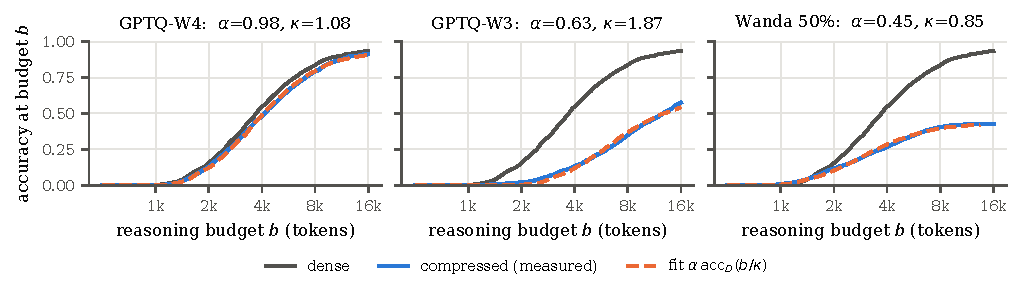
\includegraphics[width=\textwidth]{figures/budget_curves.pdf}
  \caption{Accuracy as a function of the reasoning budget for the dense Qwen3-4B and three compressed variants on MATH-500. The two-parameter fit $\alpha\,\acc_D(b/\kappa)$ (dashed) tracks the measured curve. Mild compression mainly rescales the time axis ($\kappa$); severe compression also scales it down ($\alpha$).}
  \label{fig:budget}
\end{figure}

For each compressed model $Q$ we fit $\acc_Q(b)=\alpha\,\acc_D(b/\kappa)$ by least squares on a 24-point logarithmic grid of budgets between 512 and 16,384 tokens (Figure~\ref{fig:budget}, Table~\ref{tab:alpha}). The dense curve $\acc_D$ is measured on a 400-point logarithmic grid between 64 and 16,384 tokens and interpolated linearly in $\log b$; it is set to 0 below 64 tokens and held at its 16k value above 16,384 tokens, which matters when $\kappa<1$ and $b/\kappa$ exceeds the measured range. We parameterize $\kappa=e^{\theta}$, constrain $\alpha\ge0$, and minimize with Nelder--Mead from several starting points ($\alpha\in\{0.5,1\}$, $\kappa\in\{1,2,4\}$), keeping the best solution. A compressed curve below 0.01 at every budget is assigned $\alpha=0$ with $\kappa$ undefined. Bootstrap intervals refit 200 joint resamples of problems, starting also from the point estimate. For the out-of-sample comparison, all families are fitted on the grid points up to 8,192 tokens and evaluated on the points between 8,192 and 16,384 tokens. The fit has a median RMSE of 0.007 and a maximum of 0.025 over the 51 variants. Table~\ref{tab:fitval} compares it with three other two-parameter families built on the dense curve. A power transform fits the typical variant equally well, while an additive shift and an affine map fit worse; the multiplicative time-scale form has the smallest worst-case error both in sample and when the model is fitted on budgets up to 8k and used to predict 8k--16k. We adopt it for this robustness and because it has a simple reading: $\kappa$ is the factor by which the compressed model needs more ($\kappa>1$) or fewer ($\kappa<1$) tokens to reach the same share of its final accuracy. It is an effective parameterization of the budget curve rather than a direct measurement of reasoning speed, and the power family describes the typical variant equally well. When $\alpha$ is small the compressed curve is nearly flat and $\kappa$ is not identified (the fit then reaches similar error for very different values of $\kappa$), so we report $\kappa$ only for variants with $\alpha\ge0.3$. Bootstrap intervals, which resample problems jointly for both models, exclude $\kappa=1$ for 28 of the 42 variants with an identified $\kappa$.

\begin{table}[t]
  \centering\small\setlength{\tabcolsep}{3pt}
  \adjustbox{max width=\linewidth}{\begin{tabular}{lrrrrl}
\toprule
family & median RMSE & max RMSE & median OOS & max OOS & best (in / out) \\
\midrule
dilation $\alpha\,\mathrm{acc}_D(b/\kappa)$ & 0.007 & 0.025 & 0.017 & 0.089 & 21 / 18 \\
power $\alpha\,\mathrm{acc}_D(b)^\gamma$ & 0.007 & 0.044 & 0.016 & 0.116 & 20 / 19 \\
shift $\alpha\,\mathrm{acc}_D(b-\delta)$ & 0.010 & 0.055 & 0.025 & 0.150 & 10 / 8 \\
affine $a\,\mathrm{acc}_D(b)+c$ & 0.014 & 0.083 & 0.032 & 0.201 & 0 / 6 \\
\bottomrule
\end{tabular}
}
  \caption{Two-parameter families fitted to the 51 budget curves: RMSE on the full grid, out-of-sample (OOS) error when fitting on $b\le$8k and predicting $b>$8k, and the number of variants for which each family is best.}
  \label{tab:fitval}
\end{table}

\begin{table}[t]
  \centering\small\setlength{\tabcolsep}{3pt}
  \adjustbox{max width=\linewidth}{\begin{tabular}{llrlllr}
\toprule
model & task & n & $\alpha$ (mild) & $\kappa$ (mild) & $\alpha$ (severe) & max RMSE \\
\midrule
Qwen3-1.7B & MATH & 7 & 0.50--1.01 & 0.89--1.47 & 0.00--0.08 & 0.014 \\
Qwen3-4B & MATH & 11 & 0.92--1.00 & 0.91--1.25 & 0.19--0.85 & 0.017 \\
Qwen3-8B & MATH & 11 & 0.84--1.01 & 0.96--1.24 & 0.22--0.98 & 0.014 \\
Qwen3-14B & MATH & 5 & 0.88--0.99 & 0.76--0.95 & 0.84--0.90 & 0.025 \\
Qwen3-4B & GPQA & 8 & 0.89--1.05 & 1.00--1.14 & 0.12--0.57 & 0.013 \\
R1-Llama-8B & MATH & 5 & 1.07--1.11 & 0.95--0.97 & 0.24--0.92 & 0.015 \\
Qwen3-4B & BBH & 4 & 0.94--0.94 & 1.10--1.10 & 0.10--0.87 & 0.024 \\
\bottomrule
\end{tabular}
}
  \caption{Ranges of $\alpha$ and $\kappa$ by regime and maximum fit error per model and task. Per-variant values with bootstrap intervals are in Appendix~\ref{app:tables}.}
  \label{tab:alpha}
\end{table}

Mild compression mainly rescales the budget axis. On MATH, mild variants of Qwen3-4B, 8B and 14B keep $\alpha$ between 0.84 and 1.01 while $\kappa$ ranges from 0.76 to 1.25, so some compressed models reach their accuracy with fewer tokens than the dense model and others with more. Severe compression additionally lowers the vertical scale, with $\alpha$ down to 0: within budgets up to 16k, the compressed model retains a smaller share of the dense model's accuracy. Because the curves are observed only up to 16k tokens, $\alpha$ is a finite-budget quantity rather than an asymptotic ceiling; for GPTQ-W3 on Qwen3-4B, accuracy still rises from 0.575 at 16k to 0.672 at 32k (\S\ref{sec:failure}). The severity of a given compressor depends strongly on model size: Qwen3-1.7B already collapses under 4-bit RTN ($\alpha=0.50$), whereas Qwen3-14B keeps $\alpha\ge0.84$ under 3-bit quantization. On GPQA the mild variants have point estimates of $\alpha$ between 0.89 and 1.05, but with intervals too wide to establish a lower retained accuracy.

\paragraph{Same problems?}
An aggregate curve does not show which problems a compressed model still solves. We therefore compare per-problem success at matched effective budgets: the compressed model at $b$ and the dense model at $b/\kappa$, with $b$ the largest budget for which both are measured (Appendix Table~\ref{tab:overlap}). Across the 42 variants with an identified $\kappa$, the compressed model's per-problem success covers on median 0.92 of the dense model's (range 0.36--0.99), against an aggregate ratio of 0.94; a median of 2\% of its success falls on problems where the dense model does worse, compared with 3\% between two halves of the dense model's own samples%
. For Qwen3 on MATH and BBH, the compressed model's successes are close to a subset of the dense model's: the per-problem overlap is within 0.05 of the aggregate ratio, and 0.5--6\% of the compressed model's success falls on problems the dense model solves less often, against 2--4\% between two halves of the dense model's own samples. There, $\alpha$ can be read as the share of the dense model's success that is retained. This reading fails for R1-Llama-8B, where 10--13\% of the compressed models' success falls on such problems (3.5\% for the dense model against itself), and for Qwen3-4B with GPTQ-W3 on GPQA (32\%, against 14\%): these compressed models solve partly different problems, and $\alpha$ is only an aggregate ratio.

\begin{figure}[t]
  \centering
  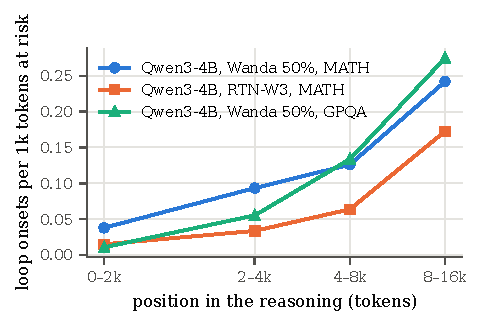
\includegraphics[width=0.62\linewidth]{figures/loop_hazard.pdf}
  \caption{Loop onsets per 1k tokens at risk, by position band, for three collapsed configurations.}
  \label{fig:hazard}
\end{figure}

\paragraph{What collapse is.}
In collapsed variants, 92--100\% of the truncated traces end in token-periodic loops with a period of at most 1,024 tokens, whereas the few truncated traces of mild variants are not loops (Appendix~\ref{app:loops}). The hazard of entering a loop increases along the trace; for Wanda-50\% on Qwen3-4B it rises from 0.04 to 0.24 onsets per 1k tokens at risk between the first 2k tokens and the 8--16k band (Figure~\ref{fig:hazard}). Except for the most damaged Qwen3-1.7B variants, loops begin late, with median onsets between 4k and 12k tokens, while dense traces end at a median of about 3.8k tokens: the compressed model first fails to conclude and then loops. Teacher-forced token divergence, measured on dense traces, decreases along the trace, so the divergence on the dense model's states does not account for the rising hazard; the divergence on the compressed model's own states, which we do not measure along the trace, may.

\section{How compressed models fail}
\label{sec:failure}

We classify every trace that does not end with a correct answer within 16k tokens as a \emph{wrong answer} (the trace terminated) or as \emph{non-terminating} (the budget ran out), and split non-terminating traces into loops (Appendix~\ref{app:loops}) and long traces without a loop. We report rates over all traces, whose denominator is fixed, and the non-terminating share of errors, which describes how a model fails independently of how often. All models of a task answer the same problems, so differences between models are bootstrapped over problems jointly.

\paragraph{Compression and the parent.}
Severe compression raises the non-termination rate in all 22 severe variants and the non-terminating share of errors in 19 of them, across both families and all three tasks (Table~\ref{tab:failure}; Appendix Table~\ref{tab:failurepaired}). Loops dominate under RTN-W3 and Wanda-50\% (81--87\% of the errors of these compressors on Qwen3-4B and of Wanda-50\% on Qwen3-8B, on MATH), whereas GPTQ-W3 produces long traces without a loop (85\% and 83\% of the errors on Qwen3-4B and Qwen3-8B). Mild compression raises the non-termination rate in 12 of 29 variants and the non-terminating share in 7 of 29. Increases above 0.06 occur only on the smallest parent, Qwen3-1.7B ($+0.10$ to $+0.47$ for its 4-bit and Wanda-30\% variants, some of which already collapse), and for per-channel RTN-W4 on Qwen3-8B ($+0.14$); on Qwen3-4B, mild variants even shift errors slightly toward wrong answers. The dense parents start from a profile in which non-termination is common: on MATH, 49--68\% of the few errors of Qwen3-1.7B, 4B and 8B are non-terminating, against 32\% [25, 39] for Qwen3-0.6B. Severe compression moves this profile further toward non-termination; for Qwen3-8B under GPTQ-W3, the error rate grows from 5\% to 20\% and the non-terminating share from 64\% to 85\%.

\paragraph{Compression versus a smaller model.}
Is a compressed model simply a weaker model? We pair each natively smaller dense model with every compressed variant whose accuracy on the same task is within 0.03 (Appendix Table~\ref{tab:matched}). When the compressed model's parent is larger than the dense model, the compressed model has the larger non-terminating share in 10 of 11 pairs. On MATH, Qwen3-0.6B (0.735) has 32\% non-terminating errors against 65\% for Qwen3-1.7B with GPTQ-W4 (0.750) and 59\% with Wanda-30\% (0.736). On GPQA-Diamond, Qwen3-0.6B (0.239) has 5\% [3, 8] against 34\% [28, 40] for Qwen3-4B with GPTQ-W3 (0.236). On BIG-Bench Hard, Qwen3-1.7B (0.758) has 1\% against 19\% [13, 26] for Qwen3-4B with GPTQ-W3 (0.783). When the parents have similar profiles, as Qwen3-4B and mild variants of Qwen3-8B and 14B, the compressed model never has the larger share (in one pair it has a smaller one). In Qwen3, a compressed model and a smaller dense model of equal accuracy are thus not interchangeable: the compressed model inherits the failure profile of its larger parent and, under severe compression, adds non-termination to it. Outside mathematics, non-termination remains a minority of the errors of moderately compressed models (19\% and 34\% for GPTQ-W3 on BIG-Bench Hard and GPQA), but dense Qwen3 models of similar accuracy almost never fail that way.

\paragraph{A different family.}
The contrast does not transfer to the R1-Distill family. R1-Qwen-1.5B, a small model distilled from the same teacher as R1-Llama-8B on a different base, reaches 0.833 on MATH with 43\% [35, 52] non-terminating errors, as many as R1-Llama-8B with GPTQ-W3 (0.754, 41\% [34, 48]) and more than its 4-bit variants (30--33\%). Non-termination therefore distinguishes compressed models from the smaller Qwen3 models, not from small reasoners in general. Both small models are distilled, but R1-Qwen-1.5B was trained only by supervised fine-tuning on the teacher's traces, whereas the small Qwen3 models were distilled from larger Qwen3 models with an on-policy stage; whether this difference explains the contrast is not tested here.

\paragraph{Budget.}
Non-termination is measured at 16k tokens, half of the output length recommended for Qwen3. To test whether it is an artifact of the budget, we let the same model continue every truncated trace by another 16k tokens with the same sampler, for 23 models and variants (all long traces without a loop and up to 200 sampled loops per variant, reweighted; Appendix Table~\ref{tab:extend}). Loops almost never resolve: 16 of 1,508 extended loops (1.1\%) terminate within the extra 16k tokens. Dense models are the opposite case: their non-termination falls from 3--8\% at 16k to at most 1.1\% at 32k, so their few truncations were mostly a matter of budget. Compressed models lie in between and keep a non-terminating share far above their parents. Loop-dominated variants (Wanda-50\%, RTN-W3) are unchanged (Qwen3-4B Wanda-50\% on MATH: 0.509 at 16k, 0.508 at 32k). GPTQ-W3, whose truncations are mostly long traces without a loop, recovers part of them, but less than the dense model: on Qwen3-4B MATH its accuracy rises from 0.575 to 0.672 and its non-termination falls from 0.380 to 0.223, against 0.961 and 0.005 for the dense model at 32k. In every one of the 12 severe variants extended, non-termination at 32k remains above the parent's rate at 16k, and the comparisons with smaller dense models at matched accuracy keep their direction (e.g., Qwen3-1.7B GPTQ-W4 at 0.803 versus Qwen3-0.6B at 0.750, with non-termination of 0.049 versus 0.010 at 32k).

\paragraph{Equal memory.}
In deployment, the alternative to a compressed model is often a smaller dense model that fits in the same memory. We compare every quantized Qwen3 variant with each smaller dense Qwen3 model whose bf16 weights take at least as much memory, on MATH (weight memory includes 16-bit group scales; unstructured sparsity is excluded because it saves no memory in dense storage; Appendix Table~\ref{tab:memory}). Of 18 pairs, the compressed model is more accurate in 2, less accurate in 10 and not distinguishable in 6; it uses more tokens per query in 12 (median ratio 1.16)%
. Calibrated 4-bit quantization (AWQ, GPTQ) of the next larger model uses 21--38\% less memory and loses at most 0.015 against the smaller dense model: Qwen3-4B with AWQ-W4 (2.7\,GB) reaches 0.929 against 0.892 for the dense Qwen3-1.7B (3.4\,GB), and Qwen3-14B with GPTQ-W4 (10.1\,GB) matches the dense Qwen3-8B (16.4\,GB; 0.945 versus 0.947) with 14\% fewer tokens; the only significant loss is for Qwen3-8B with GPTQ-W4 against the dense Qwen3-4B ($-0.015$ [$-0.030$, $-0.002$]). Uncalibrated RTN-W4 is less reliable (Qwen3-14B: $-0.094$). Every 3-bit variant is less accurate than the smaller dense model, with intervals below zero, and spends 9\% to 174\% more tokens per query; for Qwen3-8B with GPTQ-W3 against the dense Qwen3-4B, accuracy drops by 0.14 while tokens per query rise by 51\%.

\paragraph{Real kernels and scale.}
Compression in this study is simulated by dequantizing weights. For the released AWQ-W4 checkpoints of Qwen3-4B and 8B we also generate with real 4-bit kernels in vLLM. Real 4-bit kernels differ from the simulated results in at least one model (real $-$ simulated, Qwen3-4B: +0.006 [-0.006, +0.017] in accuracy and -0.002 [-0.013, +0.008] in non-termination; Qwen3-8B: -0.015 [-0.028, -0.003] in accuracy and +0.007 [-0.003, +0.018] in non-termination)%
; the difference for Qwen3-8B is small next to the effects of severe compression studied here. Qwen3-4B AWQ-W4 decodes 1.13$\times$ as fast as bf16 for a single request and 0.97$\times$ at batch 128; Qwen3-8B AWQ-W4 decodes 1.42$\times$ as fast as bf16 for a single request and 1.14$\times$ at batch 128%
. To test a larger model, we compress Qwen3-32B with RTN-W4 and Wanda-50\% and evaluate it on a fixed sample of 100 of the 300 MATH problems (Appendix Table~\ref{tab:robust}); GPTQ did not fit in the memory of a single GPU for this model, and a 3-bit RTN checkpoint did not fit in our storage quota. For Qwen3-32B, severe compression raises non-termination in 0 of 1 variants and mild compression in 0 of 1; RTN-W4 reaches 0.958 with $\alpha=0.99$ and $\kappa=1.01$; Wanda 50\% reaches 0.927 with $\alpha=0.93$ and $\kappa=0.79$%
. At this size, 50\% sparsity behaves like mild compression: the model keeps most problems ($\alpha=0.93$), reaches its accuracy with fewer tokens than the dense model ($\kappa=0.79$), its non-termination does not increase significantly, and early exit fires on 1\% of its traces. This extends the dependence of severity on model size seen from Qwen3-1.7B to Qwen3-14B: a fixed bit width or sparsity does not determine whether compression is damaging. Whether a more damaging compressor makes Qwen3-32B fail by non-termination, as it does the smaller models, is not tested here.

\begin{table}[t]
  \centering\scriptsize\setlength{\tabcolsep}{2pt}
  \adjustbox{max width=\linewidth}{\begin{tabular}{lrrlll}
\toprule
model & $\acc$ (16k) & trunc. & non-term./err. & loop/err. & long/err. \\
\midrule
Qwen3-4B + RTN-W3 & 0.181 & 0.774 & 0.95 [0.93, 0.96] & 0.87 [0.84, 0.89] & 0.08 [0.06, 0.09] \\
Qwen3-4B + Wanda 50\% & 0.427 & 0.509 & 0.89 [0.86, 0.92] & 0.86 [0.82, 0.89] & 0.03 [0.02, 0.04] \\
Qwen3-8B + Wanda 50\% & 0.504 & 0.465 & 0.94 [0.91, 0.97] & 0.81 [0.76, 0.85] & 0.13 [0.10, 0.16] \\
Qwen3-4B + GPTQ-W3 & 0.575 & 0.380 & 0.89 [0.85, 0.93] & 0.05 [0.03, 0.07] & 0.85 [0.80, 0.88] \\
Qwen3-0.6B (dense) & 0.735 & 0.085 & 0.32 [0.25, 0.39] & 0.02 [0.01, 0.04] & 0.30 [0.23, 0.36] \\
Qwen3-1.7B + Wanda 30\% & 0.736 & 0.157 & 0.59 [0.52, 0.67] & 0.13 [0.09, 0.17] & 0.46 [0.39, 0.54] \\
Qwen3-1.7B + GPTQ-W4 & 0.750 & 0.163 & 0.65 [0.57, 0.74] & 0.09 [0.05, 0.13] & 0.57 [0.48, 0.66] \\
Qwen3-8B + GPTQ-W3 & 0.797 & 0.172 & 0.85 [0.77, 0.90] & 0.02 [0.00, 0.03] & 0.83 [0.76, 0.89] \\
Qwen3-14B + Wanda 50\% & 0.835 & 0.130 & 0.79 [0.69, 0.87] & 0.24 [0.17, 0.31] & 0.55 [0.45, 0.65] \\
Qwen3-4B + RTN-W4 (per-ch.) & 0.867 & 0.076 & 0.57 [0.45, 0.68] & 0.04 [0.01, 0.08] & 0.52 [0.41, 0.64] \\
Qwen3-1.7B (dense) & 0.892 & 0.053 & 0.49 [0.36, 0.62] & 0.02 [0.00, 0.06] & 0.47 [0.34, 0.60] \\
Qwen3-4B (dense) & 0.934 & 0.045 & 0.68 [0.52, 0.84] & 0.01 [0.00, 0.04] & 0.67 [0.51, 0.83] \\
Qwen3-8B (dense) & 0.947 & 0.034 & 0.64 [0.47, 0.80] & 0.03 [0.00, 0.09] & 0.61 [0.43, 0.77] \\
\bottomrule
\end{tabular}
}
  \caption{How models fail on MATH-500 (16k budget), sorted by accuracy: accuracy, truncated share of all traces, and share of errors that did not terminate (non-term./err.), split into loops and long traces without a loop (95\% bootstrap CIs over problems). GPQA, BIG-Bench Hard and the R1-Distill family are in Appendix Table~\ref{tab:failuremore}.}
  \label{tab:failure}
\end{table}

\section{Derivation versus stopping}
\label{sec:forced}

\begin{table}[t]
  \centering\small\setlength{\tabcolsep}{2.5pt}
  \adjustbox{max width=\linewidth}{\begin{tabular}{lrrrrrr}
\toprule
model & natural 1k & forced 1k & natural 4k & forced 4k & natural 16k & forced 16k \\
\midrule
dense & 0.00 & 0.69 & 0.55 & 0.76 & 0.93 & 0.94 \\
RTN-W4 & 0.01 & 0.65 & 0.51 & 0.75 & 0.93 & 0.94 \\
GPTQ-W3 & 0.00 & 0.28 & 0.13 & 0.44 & 0.57 & 0.63 \\
Wanda 50\% & 0.01 & 0.44 & 0.27 & 0.52 & 0.43 & 0.54 \\
RTN-W3 & 0.00 & 0.23 & 0.13 & 0.32 & 0.18 & 0.29 \\
\bottomrule
\end{tabular}
}
  \caption{Natural vs.\ forced accuracy at reasoning budget $b$ (Qwen3-4B, MATH-500). ``Natural'' counts traces that finished within $b$ with a correct answer; ``forced'' closes the model's own reasoning at $b$ and requests the answer.}
  \label{tab:forced}
\end{table}

A model may fail at a given budget because its reasoning does not yet contain a recoverable answer or because it contains one but the model does not stop. To distinguish the two operationally, we close the compressed model's own reasoning at budget $b$ and request the answer (Table~\ref{tab:forced}; Qwen3-4B on MATH). Under mild compression, forced accuracy matches the dense model at every budget (RTN-W4: 0.65 versus 0.69 at 1k tokens, 0.75 versus 0.76 at 4k). Under severe compression, forcing at 16k recovers only 15--22\% of the loss: RTN-W3 improves from 0.181 to 0.293, Wanda-50\% from 0.427 to 0.541 and GPTQ-W3 from 0.575 to 0.632, against 0.934 for the dense model. Under this protocol, most of the severe-compression loss is therefore not recovered by stopping earlier: the model's own reasoning rarely yields the answer when the model is made to commit. Whether the answer was never derived or was derived but cannot be expressed is not separated by this test. The result qualifies the overthinking account of \citet{lotfi2026quantized}. For GPTQ-W3, whose dilation is the largest ($\kappa=1.87$), part of this loss is recovered by more budget: continuing the truncated traces to 32k tokens raises its accuracy to 0.672, more than forcing at 16k (0.632). For the loop-dominated compressors the opposite holds, and forcing helps more than continuing (Wanda-50\%: 0.541 forced at 16k, 0.43 at 32k). Nor does the loop make a previously recoverable answer unrecoverable: over 3,066 looped traces of compressed variants, forcing the answer at the loop onset yields 0.24 correct, against 0.23 when forcing at 16k (Appendix Table~\ref{tab:extend}). Decode-time loop breaking helps only partially: a repetition penalty of 1.1 raises Wanda-50\% to 0.59 and RTN-W3 to 0.29, and rolling back and resampling at loop onset recovers 3--15\% of looped traces (Appendix~\ref{app:interventions}).

\begin{figure}[t]
  \centering
  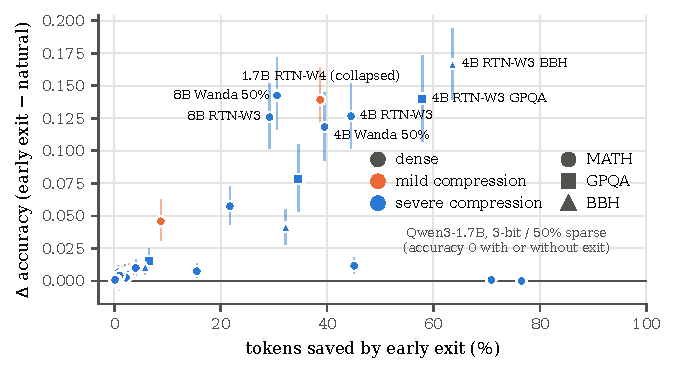
\includegraphics[width=0.7\linewidth]{figures/early_exit.pdf}
  \caption{Early exit at loop detection: change in accuracy (95\% bootstrap CI over problems) against the share of generated tokens saved, for every model and variant. No variant shows a significant loss; the gains concentrate in loop-dominated compressors, while dense and mild variants are almost unaffected.}
  \label{fig:earlyexit}
\end{figure}

\paragraph{Early exit at loop detection.}
Loops almost never resolve, and forcing the answer at the loop onset is as good as forcing it at the budget, so the tokens spent inside a loop are wasted. We therefore apply the loop criterion of Appendix~\ref{app:loops} causally: from 3,072 generated tokens on and every 256 tokens, the detector checks whether some period $p\le1{,}024$ makes the last 2,048 tokens coincide with the same tokens shifted by $p$ in at least 90\% of positions ($x_t=x_{t-p}$), and the reasoning is closed with the end-of-thinking marker as soon as this holds, after which the answer is generated with at most 768 tokens. Because the prefix up to that point is the recorded trace, the policy can be evaluated on the existing generations by generating only the forced answer; the detector fires on average about 1.8k tokens after the loop onset. Early exit lowers the point estimate of accuracy in 2 of the 67 models and variants (by at most 0.003) and none significantly: no 95\% interval lies entirely below zero, and the lowest lower bound of the per-variant intervals is -0.0075; these are marginal intervals, not a simultaneous bound on the loss across variants, and the absence of a significant loss is not a demonstration of equivalence. On the 14 dense models, accuracy changes by at most +0.005 and the detector fires on at most 1.1\% of traces. Under severe compression, accuracy rises in 18 of 23 variants while generation uses up to 77\% fewer tokens. The gains concentrate in the loop-dominated compressors: for Qwen3-4B and 8B with RTN-W3 and Wanda-50\%, accuracy rises by +0.042 to +0.167 with 29--64\% fewer tokens, whereas GPTQ-W3 changes by at most +0.015. False positives, traces on which the detector fires that would have ended with a correct answer, are at most 2.9\% of traces%
 (Figure~\ref{fig:earlyexit}; Appendix Table~\ref{tab:earlyexit}).

Section~\ref{sec:swap} shows the other side: a severely compressed model answers well when the dense model's reasoning is supplied, even though its own reasoning rarely yields the answer.

\section{What compression does not change: reading versus writing}
\label{sec:swap}

\begin{figure}[t]
  \centering
  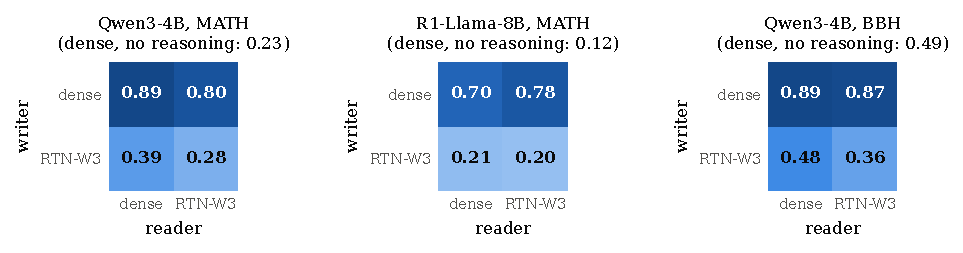
\includegraphics[width=\textwidth]{figures/matrix.pdf}
  \caption{Accuracy for each writer--reader pair (4k reasoning tokens, answers capped at 32 tokens) in three settings. Changing the writer (rows) costs far more than changing the reader (columns). The titles give the dense model's accuracy with no reasoning.}
  \label{fig:matrix}
\end{figure}

\paragraph{Protocol.}
A \emph{writer} produces 4,096 tokens of reasoning; the reasoning block is closed and a \emph{reader} answers immediately, continuing from ``The final answer is \texttt{\textbackslash boxed\{}'' with at most 32 tokens. We write $\accwr{W}{R}$ for the accuracy with writer $W$ and reader $R$, and define for a dense model $D$ and its compressed copy $Q$
\begin{equation*}
\begin{aligned}
\text{writing damage} &= \accwr{D}{D}-\accwr{Q}{D},\\
\text{reading damage} &= \accwr{D}{D}-\accwr{D}{Q}.
\end{aligned}
\end{equation*}
Writing damage holds the dense reader fixed and changes the writer; reading damage holds the dense reasoning fixed and changes the reader. The answer cap is required for these quantities to be interpretable. With a free answer of up to 2,048 tokens, Qwen3 readers re-solve the problem in the answer itself, so that the dense Qwen3-4B reaches 0.84 on MATH with no reasoning at all. Under the cap the dense reader without reasoning scores between 0.12 and 0.39, depending on model and task, and accuracy reflects what the reasoning carries. Results under the free answer are reported in Appendix~\ref{app:tables} for completeness.

\begin{figure}[t]
  \centering
  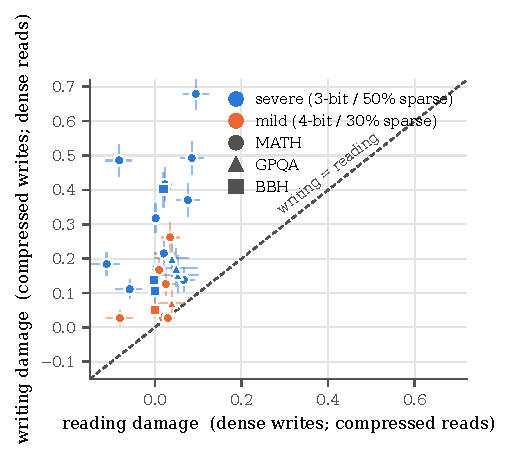
\includegraphics[width=0.62\linewidth]{figures/write_read.pdf}
  \caption{Writing vs.\ reading damage for 24 model--compressor--task combinations, with 95\% CIs. Points above the diagonal indicate that the compressed model is a worse writer than reader.}
  \label{fig:writeread}
\end{figure}

\paragraph{Writing damage dominates.}
Figures~\ref{fig:matrix} and~\ref{fig:writeread} summarize the result. Writing damage exceeds reading damage in 21/24 combinations after Holm correction, including all 16 severe ones across both model families and all three tasks (Appendix Table~\ref{tab:writeread}). For severe compressors, writing damage ranges from 0.11 to 0.68, whereas reading damage never exceeds 0.094; for R1-Llama-8B it is negative ($-0.06$ to $-0.11$), meaning that compressed readers extract more from dense reasoning than the dense model itself. The three exceptions are mild 4-bit RTN variants, for which both damages are small. Given dense reasoning, severely compressed Qwen3 models close 67--100\% of their gap to the dense model on MATH; Qwen3-4B with RTN-W3, for example, rises from 0.28 when reading its own reasoning to 0.80 when reading the dense model's, against 0.89 for the dense model.

\paragraph{Control for budget dilation.}
A 4k-token prefix written by a model with $\kappa>1$ covers less of the reasoning than 4k tokens of the dense model, so part of the writing damage could reflect slower progress rather than worse reasoning. We therefore compare each compressed prefix with a dense prefix of $4096/\kappa$ tokens, interpolating the dense writer's accuracy between the measured budgets of 1k, 2k and 4k tokens (for $\kappa\le1$ we keep 4k, which is conservative). For severe compressors, matching reduces writing damage by at most about a quarter: for Qwen3-4B with GPTQ-W3 ($\kappa=1.87$), it goes from 0.37 to 0.29 [0.24, 0.33], against a reading damage of 0.08. The same 21 of 24 combinations retain a writing damage larger than the reading damage (Appendix Table~\ref{tab:dilation}).

\paragraph{Control for answer leakage.}
Cross-model transfer can be driven by answer leakage \citep{cheng2026travels}, and 4k-token dense prefixes often state the answer, in which case reading reduces to copying. We repeat the decomposition at 1k, 2k and 4k tokens, restricted to dense prefixes that contain neither \texttt{\textbackslash boxed\{} nor the gold answer string (Appendix Table~\ref{tab:leak}). Leakage does inflate the apparent reading ability: on non-leaked MATH prefixes, reading damage reaches 0.24, compared with at most 0.14 over all prefixes. The asymmetry nonetheless grows with reasoning length while reading damage stays roughly constant; for Qwen3-4B with RTN-W3, writing damage rises from 0.18 to 0.30 and 0.42 at 1k, 2k and 4k tokens, while reading damage is 0.24, 0.24 and 0.16. At 4k tokens the asymmetry holds on non-leaked prefixes in 12 of 13 severe MATH and GPQA combinations. At 1k tokens the picture is mixed: writing damage is larger in 5 combinations, the two do not differ in 6, and reading damage is larger in 2. On BBH, where 92\% of dense reasoning is complete within 4k tokens, we restrict to dense reasoning that is still incomplete at the budget; writing damage exceeds reading damage at every budget for every compressor (11 of 12 intervals exclude zero). The string-based leakage test misses equivalent forms of an answer (e.g., $0.5$ and $\frac12$) and therefore underestimates leakage.

\paragraph{Is the asymmetry specific to compression?}
Weaker models are known to benefit from the reasoning of stronger ones \citep{cheng2026travels}, so the asymmetry may reflect weakness in general rather than compression. We repeat the swap with natively smaller dense models of the same family (Qwen3-0.6B, 1.7B and 4B as weak models; 1.7B, 4B and 8B as strong ones), which share the tokenizer (Appendix Table~\ref{tab:densepairs}). The asymmetry appears there as well: writing damage exceeds reading damage in all six dense pairs. At matched accuracy of the weak model when it writes and reads its own reasoning, the two kinds of weak model are indistinguishable: Qwen3-0.6B paired with Qwen3-8B (own accuracy 0.61) has a writing damage of 0.20 and a reading damage of 0.05, while Qwen3-8B with Wanda-50\% (0.63) and with GPTQ-W3 (0.67) have 0.22 and 0.02, and 0.14 and 0.07. The writing--reading asymmetry is therefore a property of weaker reasoners, and compression places a model on the same curve as a smaller one; what distinguishes compression in Qwen3 is how the model fails (\S\ref{sec:failure}).

\paragraph{Information in compressed reasoning.}
Relative to answering with no reasoning, the dense reader still gains from compressed reasoning on MATH: typically about half of the gain it obtains from its own reasoning, and 16--29\% for RTN-W3 writers. On GPQA, reasoning written by severe compressors yields no gain.

\paragraph{An interventional test.}
When the dense model writes about 10\% of the compressed model's tokens, frequent short chunks help more than infrequent long ones for the two loop-collapse compressors ($+0.068$ and $+0.103$ for 50- versus 400-token chunks), but not for GPTQ-W3. This is consistent with compounding errors, but frequent chunks also interrupt loops before they settle, so the test does not isolate the mechanism (Appendix~\ref{sec:ablation}).

\paragraph{Sampling noise.}
Compressed models are far more sensitive to the sampling temperature than the dense model, and lower temperatures increase looping; raising the dense model's temperature, however, does not reproduce compression damage under standard decoding settings (Appendix~\ref{sec:temperature}).

\section{Negative results}
\label{sec:negative}

Several attempts to predict compression damage without generation were unsuccessful, and we report them because they bound what such metrics can claim. Per-token KL and total variation under teacher forcing rank the collapse loss well (pooled Spearman 0.93--0.94 over 23 variants), and a cheap probe of 1k-token continuations reaches 0.97, but none of these quantities predicts $\kappa$ in the mild regime ($|\rho|\le0.58$). An estimator of the accuracy change based on the performance-difference lemma \citep{kakade2002approximately}, with forks sampled in proportion to the token-level divergence, has variance orders of magnitude above the signal. Damage is not a single function of divergence multiplied by reasoning length.

We also pre-registered a rule derived from development data: thinking protects compressed models when the token-level total variation is below 0.114 and amplifies damage above it. The rule, the metrics, the held-out set and the success criteria were fixed in a dated file before the held-out data were generated (Appendix~\ref{app:prereg}). On the held-out models and compressors, the predicted sign was correct for 9 of 10 points, but the pre-registered monotonicity criterion failed (Spearman $+0.81$ instead of at most $-0.6$), no held-out point fell above the threshold, and Qwen3-14B with RTN-W4 is a clear counterexample. The threshold is therefore not claimed.

\section{Implications}

Compressed reasoning models should be evaluated on budget curves rather than on a single accuracy value: one long generation per model yields $\alpha$ and $\kappa$, which distinguish a compressed model that needs a different budget from one that retains less of the dense model's accuracy within the budget. In Qwen3, a compressed model and a smaller dense model of equal accuracy are not interchangeable: the compressed model inherits its parent's failure profile and, under severe compression, adds non-termination, which a single accuracy value hides. Because forcing an answer recovers little of this loss, remedies should target the progress of the reasoning itself, for instance by training on the model's own trajectories, rather than only the decision to stop. When memory is the constraint, calibrated 4-bit quantization of a larger model is close to or better than a smaller dense model, whereas 3-bit quantization is not, and its cost appears in tokens as well as in accuracy. Since loops are detectable while they form, closing the reasoning at detection is a cheap default for compressed deployments: in our evaluation it saved tokens and never lowered accuracy significantly. Teacher-forced fidelity metrics evaluate a compressed model on the dense model's states, the setting closest to our reading condition; they rank damage but do not capture the larger damage we observe when the model writes its own reasoning, which supports evaluating and training compressed reasoners on their own trajectories \citep{chen2026onpolicy,zheng2026rightonq}. The preserved reading ability may also explain why routing a small fraction of tokens or steps to a stronger model recovers accuracy \citep{huang2026relayllm,akhauri2025splitreason}; for collapse-type damage, the timing of such interventions matters in addition to their amount.

\section{Limitations}

The study covers two model families and math, science and BIG-Bench Hard tasks, but no code generation; the failure-mode contrast with natively smaller models holds for Qwen3 on three tasks but not for a small R1-distilled model, and the swap with smaller dense models covers only Qwen3 on MATH; BIG-Bench Hard, the forced answer and the interventional test were run only on Qwen3-4B. All generations use a 16k-token budget, half of the length recommended for Qwen3; extending truncated traces to 32k leaves the conclusions unchanged, but for GPTQ-W3 a substantial part of the 16k non-termination resolves, and budgets beyond 32k were not tested. The severity rule is a priori in the sense that it depends only on bit width and sparsity, but it was not registered before the experiments. The Qwen3-32B check uses 100 of the 300 MATH problems, a single task and only two compressors, because GPTQ and a third checkpoint did not fit in our GPU memory and storage. Compression is simulated and weight-only, except for a check with real 4-bit AWQ kernels; activation and KV-cache quantization are not studied, and each configuration uses a single calibration run. Weight memory in the equal-memory comparison is computed from bit width and group size, not measured. The early-exit policy is evaluated on recorded traces with a single detector setting that was not tuned, and the absence of a significant loss is not a guarantee for other models or tasks. The forced answer measures whether an answer can be recovered under one prompting protocol and does not identify whether the model derived it internally; similarly, $\kappa$ and $\alpha$ summarize budget curves and are not direct measurements of reasoning speed or of which problems are solved (Section~\ref{sec:budget} reports the per-problem overlap). The 32-token answer cap removes re-solving but may penalize readers that need a few verification steps, and the leakage test is string-based and approximate. The interventional test is consistent with compounding errors but does not separate them from loop interruption, and the infrequent schedules ended with a slightly lower dense share (8.6--9.5\% versus 9.7\%). Most analyses use four samples per problem (two in the interventional test). The study used about 260 H100 GPU-hours: 193 recorded by the cluster scheduler and an estimated 60--70 in early unscheduled runs.

\bibliographystyle{tmlr}
\bibliography{references}

\appendix

\section{An interventional test}
\label{sec:ablation}

\begin{figure}[t]
  \centering
  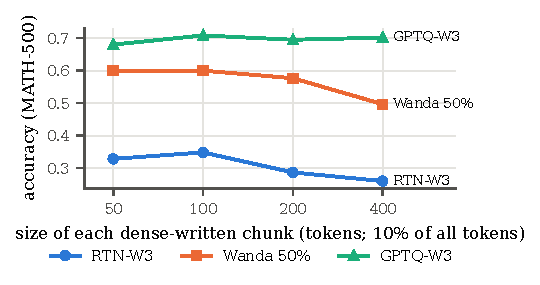
\includegraphics[width=0.62\linewidth]{figures/ablation.pdf}
  \caption{Accuracy when the dense model writes about 10\% of the tokens in chunks of different size (Qwen3-4B, MATH-500, two samples per problem).}
  \label{fig:ablation}
\end{figure}

If compressed models fail by compounding their own deviations, the frequency of corrections should matter at a fixed amount of correction. We let the dense model write about 10\% of the tokens of the compressed model's reasoning, in chunks of 50, 100, 200 or 400 tokens, within one shared 16k budget (Qwen3-4B, MATH; Figure~\ref{fig:ablation}). For the two compressors whose failure is collapse into loops, frequent corrections outperform infrequent ones at the same dense share: chunks of 50 versus 400 tokens yield $+0.068$ [$+0.030$, $+0.107$] for RTN-W3 and $+0.103$ [$+0.065$, $+0.143$] for Wanda-50\%. For GPTQ-W3, whose failure is dilation ($\kappa=1.87$) rather than looping, the difference is $-0.022$ [$-0.047$, $+0.003$]. These results are consistent with compounding errors for loop-collapse compressors, but they do not isolate the mechanism: frequent dense chunks also interrupt loops before they settle, which would produce the same pattern. The intervention itself is modest, recovering 10--37\% of the gap with about 10\% of dense tokens.

\section{Compression and sampling noise}
\label{sec:temperature}

The dense Qwen3-4B is insensitive to the sampling temperature between 0.3 and 1.3 (accuracy 0.933--0.940), whereas compressed models are not (Appendix Table~\ref{tab:temp}). Lower temperatures increase looping: for GPTQ-W3, the share of truncated traces that are loops rises from 5\% to 61\% at temperature 0.3. Higher temperatures help the looping compressors: Wanda-50\% scores 0.27, 0.43 and 0.58 at temperatures 0.3, 0.6 and 1.0, and RTN-W3 0.08, 0.18 and 0.25, whereas GPTQ-W3 barely changes above 0.6 (0.57 and 0.60). Compressed models were not run at temperature 1.3. Under teacher forcing every compressed model is flatter than the dense one (effective temperature between 1.1 and 2.0), yet raising the dense model's temperature within this range does not reproduce compression damage. Because all runs use top-$k$ and top-$p$ truncation, which bounds the noise a higher temperature can inject, this shows only that the damage is not reproduced by temperature under standard decoding settings; it does not rule out other forms of noise.


\section{Additional tables}
\label{app:tables}

\begin{table}[t]
  \centering\footnotesize\setlength{\tabcolsep}{4pt}
  \adjustbox{max width=\linewidth}{\begin{tabular}{llllll}
\toprule
model & task & compressor & writing damage & reading damage & writing $-$ reading \\
\midrule
Qwen3-1.7B & MATH & RTN-W4 & +0.261 [+0.223, +0.304] & +0.035 [+0.014, +0.058] & +0.226 [+0.185, +0.270] \\
Qwen3-1.7B & MATH & GPTQ-W4 & +0.167 [+0.132, +0.206] & +0.011 [-0.007, +0.030] & +0.156 [+0.117, +0.196] \\
Qwen3-1.7B & MATH & Wanda 30\% & +0.126 [+0.092, +0.158] & +0.025 [+0.006, +0.047] & +0.100 [+0.062, +0.137] \\
Qwen3-1.7B & MATH & GPTQ-W3 & +0.679 [+0.639, +0.723] & +0.094 [+0.069, +0.123] & +0.585 [+0.537, +0.630] \\
Qwen3-4B & MATH & RTN-W4 & +0.029 [+0.011, +0.047] & +0.018 [+0.006, +0.032] & +0.010 [-0.011, +0.032] \\
Qwen3-4B & MATH & GPTQ-W3 & +0.369 [+0.324, +0.418] & +0.076 [+0.049, +0.103] & +0.293 [+0.246, +0.343] \\
Qwen3-4B & MATH & Wanda 50\% & +0.317 [+0.273, +0.362] & +0.002 [-0.011, +0.016] & +0.315 [+0.269, +0.359] \\
Qwen3-4B & MATH & RTN-W3 & +0.492 [+0.443, +0.536] & +0.085 [+0.058, +0.113] & +0.407 [+0.355, +0.457] \\
Qwen3-8B & MATH & RTN-W4 & +0.027 [+0.010, +0.043] & +0.030 [+0.015, +0.046] & -0.003 [-0.025, +0.019] \\
Qwen3-8B & MATH & GPTQ-W3 & +0.139 [+0.104, +0.176] & +0.067 [+0.042, +0.093] & +0.072 [+0.032, +0.112] \\
Qwen3-8B & MATH & Wanda 50\% & +0.215 [+0.177, +0.255] & +0.020 [-0.002, +0.043] & +0.194 [+0.153, +0.236] \\
Qwen3-8B & MATH & RTN-W3 & +0.417 [+0.370, +0.462] & +0.023 [+0.008, +0.039] & +0.393 [+0.345, +0.439] \\
Qwen3-4B & GPQA & RTN-W4 & +0.072 [+0.037, +0.109] & +0.039 [+0.009, +0.071] & +0.034 [-0.008, +0.075] \\
Qwen3-4B & GPQA & GPTQ-W3 & +0.152 [+0.098, +0.205] & +0.054 [+0.008, +0.101] & +0.098 [+0.033, +0.163] \\
Qwen3-4B & GPQA & Wanda 50\% & +0.201 [+0.148, +0.258] & +0.038 [+0.003, +0.077] & +0.162 [+0.102, +0.221] \\
Qwen3-4B & GPQA & RTN-W3 & +0.173 [+0.115, +0.230] & +0.049 [+0.000, +0.100] & +0.124 [+0.058, +0.188] \\
R1-Llama-8B & MATH & RTN-W4 & +0.026 [+0.007, +0.049] & -0.080 [-0.109, -0.052] & +0.107 [+0.074, +0.139] \\
R1-Llama-8B & MATH & GPTQ-W3 & +0.112 [+0.085, +0.140] & -0.058 [-0.087, -0.029] & +0.169 [+0.132, +0.207] \\
R1-Llama-8B & MATH & Wanda 50\% & +0.185 [+0.151, +0.219] & -0.111 [-0.144, -0.081] & +0.296 [+0.255, +0.337] \\
R1-Llama-8B & MATH & RTN-W3 & +0.484 [+0.439, +0.530] & -0.083 [-0.115, -0.053] & +0.568 [+0.522, +0.611] \\
Qwen3-4B & BBH & RTN-W4 & +0.050 [+0.027, +0.075] & +0.000 [-0.004, +0.005] & +0.050 [+0.028, +0.076] \\
Qwen3-4B & BBH & GPTQ-W3 & +0.108 [+0.075, +0.142] & +0.000 [-0.005, +0.005] & +0.108 [+0.075, +0.142] \\
Qwen3-4B & BBH & Wanda 50\% & +0.137 [+0.096, +0.178] & -0.002 [-0.009, +0.003] & +0.140 [+0.098, +0.181] \\
Qwen3-4B & BBH & RTN-W3 & +0.403 [+0.353, +0.455] & +0.020 [+0.007, +0.035] & +0.383 [+0.331, +0.436] \\
\bottomrule
\end{tabular}
}
  \caption{Writing and reading damage with 95\% bootstrap CIs (4k reasoning tokens, answers capped at 32 tokens).}
  \label{tab:writeread}
\end{table}

\begin{table}[t]
  \centering\scriptsize\setlength{\tabcolsep}{3pt}
  \adjustbox{max width=\linewidth}{\begin{tabular}{llrrlll}
\toprule
strong & weak & weak alone (acc) & strong alone (acc) & writing damage & reading damage & writing - reading \\
\midrule
Qwen3-8B & Qwen3-1.7B (dense) & 0.82 & 0.87 & +0.068 [+0.045, +0.091] & -0.003 [-0.022, +0.014] & +0.072 [+0.045, +0.098] \\
Qwen3-4B & Qwen3-1.7B (dense) & 0.82 & 0.89 & +0.052 [+0.027, +0.077] & +0.013 [+0.001, +0.029] & +0.038 [+0.012, +0.066] \\
Qwen3-8B & Qwen3-4B (dense) & 0.89 & 0.87 & +0.010 [-0.007, +0.027] & -0.017 [-0.034, -0.003] & +0.027 [+0.007, +0.048] \\
Qwen3-8B & Qwen3-0.6B (dense) & 0.61 & 0.87 & +0.199 [+0.165, +0.234] & +0.051 [+0.023, +0.080] & +0.148 [+0.104, +0.190] \\
Qwen3-4B & Qwen3-0.6B (dense) & 0.61 & 0.89 & +0.204 [+0.169, +0.242] & +0.074 [+0.048, +0.104] & +0.130 [+0.086, +0.175] \\
Qwen3-1.7B & Qwen3-0.6B (dense) & 0.61 & 0.82 & +0.150 [+0.119, +0.183] & +0.071 [+0.046, +0.098] & +0.079 [+0.039, +0.118] \\
Qwen3-4B & Qwen3-4B + RTN-W4 & 0.84 & 0.89 & +0.029 [+0.013, +0.047] & +0.018 [+0.006, +0.032] & +0.011 [-0.011, +0.033] \\
Qwen3-4B & Qwen3-4B + GPTQ-W3 & 0.46 & 0.89 & +0.369 [+0.320, +0.419] & +0.076 [+0.050, +0.104] & +0.293 [+0.244, +0.343] \\
Qwen3-4B & Qwen3-4B + Wanda 50\% & 0.55 & 0.89 & +0.317 [+0.274, +0.360] & +0.002 [-0.012, +0.015] & +0.315 [+0.272, +0.359] \\
Qwen3-4B & Qwen3-4B + RTN-W3 & 0.28 & 0.89 & +0.493 [+0.447, +0.542] & +0.085 [+0.058, +0.116] & +0.407 [+0.356, +0.462] \\
Qwen3-8B & Qwen3-8B + RTN-W4 & 0.81 & 0.87 & +0.027 [+0.011, +0.042] & +0.030 [+0.015, +0.047] & -0.003 [-0.026, +0.018] \\
Qwen3-8B & Qwen3-8B + GPTQ-W3 & 0.67 & 0.87 & +0.139 [+0.105, +0.174] & +0.066 [+0.042, +0.093] & +0.073 [+0.032, +0.112] \\
Qwen3-8B & Qwen3-8B + Wanda 50\% & 0.62 & 0.87 & +0.215 [+0.176, +0.253] & +0.021 [-0.001, +0.046] & +0.193 [+0.152, +0.237] \\
Qwen3-8B & Qwen3-8B + RTN-W3 & 0.35 & 0.87 & +0.416 [+0.372, +0.463] & +0.023 [+0.007, +0.040] & +0.393 [+0.347, +0.442] \\
\bottomrule
\end{tabular}
}
  \caption{Writer$\times$reader decomposition for natively smaller dense models and for compressed copies (MATH-500, 4k reasoning tokens, short answers). ``Alone'' is the accuracy of a model writing and reading its own reasoning.}
  \label{tab:densepairs}
\end{table}

\begin{table}[t]
  \centering\scriptsize\setlength{\tabcolsep}{3pt}
  \adjustbox{max width=\linewidth}{\begin{tabular}{llrrlll}
\toprule
model & task & $\acc$ (16k) & trunc. & non-term./err. & loop/err. & long/err. \\
\midrule
Qwen3-4B + RTN-W3 & GPQA & 0.067 & 0.784 & 0.84 [0.80, 0.88] & 0.81 [0.78, 0.85] & 0.03 [0.02, 0.04] \\
Qwen3-4B + Wanda 50\% & GPQA & 0.144 & 0.477 & 0.56 [0.49, 0.62] & 0.54 [0.48, 0.60] & 0.02 [0.01, 0.03] \\
Qwen3-4B + GPTQ-W3 & GPQA & 0.236 & 0.258 & 0.34 [0.28, 0.40] & 0.19 [0.15, 0.24] & 0.14 [0.10, 0.19] \\
Qwen3-0.6B (dense) & GPQA & 0.239 & 0.040 & 0.05 [0.03, 0.08] & 0.01 [0.01, 0.03] & 0.04 [0.02, 0.06] \\
Qwen3-1.7B (dense) & GPQA & 0.321 & 0.105 & 0.16 [0.11, 0.20] & 0.01 [0.00, 0.01] & 0.15 [0.10, 0.20] \\
Qwen3-4B + RTN-W4 & GPQA & 0.441 & 0.067 & 0.12 [0.07, 0.17] & 0.01 [0.00, 0.03] & 0.11 [0.06, 0.16] \\
Qwen3-4B + Wanda 30\% & GPQA & 0.455 & 0.095 & 0.17 [0.12, 0.24] & 0.02 [0.01, 0.05] & 0.15 [0.10, 0.21] \\
Qwen3-4B + AWQ-W4 & GPQA & 0.481 & 0.078 & 0.15 [0.10, 0.21] & 0.02 [0.00, 0.04] & 0.13 [0.08, 0.19] \\
Qwen3-4B + GPTQ-W4 & GPQA & 0.484 & 0.080 & 0.15 [0.10, 0.21] & 0.01 [0.00, 0.02] & 0.14 [0.10, 0.20] \\
Qwen3-4B (dense) & GPQA & 0.515 & 0.083 & 0.17 [0.11, 0.23] & 0.01 [0.00, 0.03] & 0.16 [0.10, 0.22] \\
Qwen3-4B + RTN-W8 & GPQA & 0.516 & 0.072 & 0.15 [0.10, 0.21] & 0.02 [0.00, 0.04] & 0.13 [0.08, 0.18] \\
Qwen3-4B + RTN-W3 & BBH & 0.093 & 0.775 & 0.86 [0.82, 0.88] & 0.81 [0.78, 0.84] & 0.04 [0.03, 0.05] \\
Qwen3-0.6B (dense) & BBH & 0.551 & 0.001 & 0.00 [0.00, 0.01] & 0.00 [0.00, 0.00] & 0.00 [0.00, 0.01] \\
Qwen3-4B + Wanda 50\% & BBH & 0.689 & 0.121 & 0.39 [0.32, 0.46] & 0.39 [0.31, 0.46] & 0.01 [0.00, 0.01] \\
Qwen3-1.7B (dense) & BBH & 0.758 & 0.003 & 0.01 [0.00, 0.02] & 0.00 [0.00, 0.00] & 0.01 [0.00, 0.02] \\
Qwen3-4B + GPTQ-W3 & BBH & 0.783 & 0.042 & 0.19 [0.13, 0.26] & 0.12 [0.08, 0.17] & 0.07 [0.03, 0.12] \\
Qwen3-4B + RTN-W4 & BBH & 0.828 & 0.003 & 0.01 [0.00, 0.03] & 0.00 [0.00, 0.02] & 0.01 [0.00, 0.03] \\
Qwen3-4B (dense) & BBH & 0.878 & 0.001 & 0.01 [0.00, 0.02] & 0.00 [0.00, 0.00] & 0.01 [0.00, 0.02] \\
R1-Llama-8B + RTN-W3 & MATH & 0.193 & 0.223 & 0.27 [0.24, 0.31] & 0.21 [0.18, 0.24] & 0.06 [0.05, 0.08] \\
R1-Llama-8B + Wanda 50\% & MATH & 0.546 & 0.303 & 0.67 [0.62, 0.72] & 0.56 [0.51, 0.60] & 0.11 [0.08, 0.14] \\
R1-Llama-8B + GPTQ-W3 & MATH & 0.754 & 0.100 & 0.41 [0.34, 0.48] & 0.09 [0.05, 0.13] & 0.32 [0.24, 0.39] \\
R1-Llama-8B (dense) & MATH & 0.804 & 0.037 & 0.19 [0.12, 0.26] & 0.01 [0.00, 0.03] & 0.17 [0.11, 0.25] \\
R1-Qwen-1.5B (dense) & MATH & 0.833 & 0.072 & 0.43 [0.35, 0.52] & 0.04 [0.02, 0.07] & 0.39 [0.31, 0.48] \\
R1-Llama-8B + RTN-W4 & MATH & 0.868 & 0.040 & 0.30 [0.22, 0.39] & 0.05 [0.02, 0.09] & 0.25 [0.17, 0.34] \\
R1-Llama-8B + GPTQ-W4 & MATH & 0.887 & 0.037 & 0.33 [0.23, 0.43] & 0.05 [0.02, 0.09] & 0.28 [0.19, 0.37] \\
\bottomrule
\end{tabular}
}
  \caption{How models fail on GPQA-Diamond and BIG-Bench Hard (Qwen3) and on MATH-500 (R1-Distill family), 16k budget, sorted by accuracy within each block. Columns as in Table~\ref{tab:failure}. R1-Qwen-1.5B is DeepSeek-R1-Distill-Qwen-1.5B, a dense model distilled from the same teacher as R1-Llama-8B.}
  \label{tab:failuremore}
\end{table}

\begin{table}[t]
  \centering\scriptsize\setlength{\tabcolsep}{3pt}
  \adjustbox{max width=\linewidth}{\begin{tabular}{lllrrrrrr}
\toprule
task & model & compressor & $\acc$ 16k & $\acc$ 32k & non-term. 16k & non-term. 32k & loops/cut & forced onset / 16k \\
\midrule
MATH & Qwen3-0.6B & dense & 0.735 & 0.750 & 0.085 & 0.010 & 0.07 & -- \\
MATH & Qwen3-1.7B & dense & 0.892 & 0.910 & 0.053 & 0.009 & 0.05 & -- \\
MATH & Qwen3-1.7B & GPTQ-W4 & 0.750 & 0.803 & 0.163 & 0.049 & 0.13 & 0.27 / 0.27 \\
MATH & Qwen3-1.7B & Wanda 30\% & 0.736 & 0.767 & 0.157 & 0.068 & 0.22 & 0.27 / 0.34 \\
MATH & Qwen3-4B & dense & 0.934 & 0.961 & 0.045 & 0.005 & 0.02 & -- \\
MATH & Qwen3-4B & RTN-W4 (per-ch.) & 0.867 & 0.886 & 0.076 & 0.010 & 0.08 & -- \\
MATH & Qwen3-4B & GPTQ-W3 & 0.575 & 0.672 & 0.380 & 0.223 & 0.05 & 0.32 / 0.28 \\
MATH & Qwen3-4B & Wanda 50\% & 0.427 & 0.427 & 0.509 & 0.508 & 0.97 & 0.24 / 0.24 \\
MATH & Qwen3-4B & RTN-W3 & 0.181 & 0.185 & 0.774 & 0.748 & 0.92 & 0.18 / 0.16 \\
MATH & Qwen3-8B & dense & 0.947 & 0.962 & 0.034 & 0.007 & 0.05 & -- \\
MATH & Qwen3-8B & GPTQ-W3 & 0.797 & 0.863 & 0.172 & 0.068 & 0.02 & -- \\
MATH & Qwen3-8B & Wanda 50\% & 0.504 & 0.509 & 0.465 & 0.457 & 0.86 & 0.34 / 0.34 \\
MATH & Qwen3-14B & Wanda 50\% & 0.835 & 0.870 & 0.130 & 0.078 & 0.30 & 0.34 / 0.34 \\
MATH & R1-Llama-8B & dense & 0.804 & 0.815 & 0.037 & 0.004 & 0.07 & -- \\
MATH & R1-Llama-8B & GPTQ-W3 & 0.754 & 0.776 & 0.100 & 0.045 & 0.23 & 0.19 / 0.15 \\
MATH & R1-Llama-8B & Wanda 50\% & 0.546 & 0.546 & 0.303 & 0.302 & 0.84 & 0.21 / 0.22 \\
MATH & R1-Qwen-1.5B & dense & 0.833 & 0.841 & 0.072 & 0.027 & 0.09 & -- \\
GPQA & Qwen3-0.6B & dense & 0.239 & 0.250 & 0.040 & 0.011 & 0.28 & -- \\
GPQA & Qwen3-4B & dense & 0.515 & 0.549 & 0.083 & 0.011 & 0.08 & -- \\
GPQA & Qwen3-4B & GPTQ-W3 & 0.236 & 0.247 & 0.258 & 0.221 & 0.58 & 0.13 / 0.10 \\
GPQA & Qwen3-4B & Wanda 50\% & 0.144 & 0.144 & 0.477 & 0.477 & 0.97 & 0.21 / 0.18 \\
BBH & Qwen3-4B & GPTQ-W3 & 0.783 & 0.787 & 0.042 & 0.033 & 0.64 & 0.38 / 0.28 \\
BBH & Qwen3-4B & Wanda 50\% & 0.689 & 0.689 & 0.121 & 0.121 & 0.99 & 0.42 / 0.34 \\
\bottomrule
\end{tabular}
}
  \caption{Truncated traces continued from 16k to 32k tokens by the same model and sampler. Accuracy and non-terminating share of all traces at 16k (measured) and 32k (estimated: all long traces without a loop are extended, loops are subsampled to at most 200 and reweighted). ``loops/cut'' is the share of 16k-truncated traces that are loops. The last column gives the accuracy of a forced answer on looped traces, closing the reasoning at the loop onset versus at 16k (shown when at least 10 loops).}
  \label{tab:extend}
\end{table}

\begin{table}[t]
  \centering\scriptsize\setlength{\tabcolsep}{3pt}
  \adjustbox{max width=\linewidth}{\begin{tabular}{lllrrrrrrr}
\toprule
model & task & compressor & $\kappa$ & ratio & overlap & novel & $\rho$ & novel (self) & $\rho$ (self) \\
\midrule
Qwen3-1.7B & MATH & RTN-W8 & 1.02 & 1.01 & 0.98 & 0.03 & 0.88 & 0.04 & 0.76 \\
Qwen3-1.7B & MATH & GPTQ-W4 & 1.47 & 0.89 & 0.85 & 0.05 & 0.65 & 0.04 & 0.76 \\
Qwen3-1.7B & MATH & RTN-W4 & 0.89 & 0.48 & 0.47 & 0.01 & 0.39 & 0.04 & 0.76 \\
Qwen3-1.7B & MATH & Wanda 30\% & 1.01 & 0.83 & 0.82 & 0.01 & 0.65 & 0.04 & 0.76 \\
Qwen3-4B & MATH & RTN-W8 & 1.00 & 1.01 & 0.99 & 0.02 & 0.86 & 0.02 & 0.75 \\
Qwen3-4B & MATH & AWQ-W4 & 0.91 & 0.99 & 0.97 & 0.02 & 0.82 & 0.02 & 0.75 \\
Qwen3-4B & MATH & GPTQ-W4 & 1.08 & 0.98 & 0.97 & 0.01 & 0.85 & 0.02 & 0.75 \\
Qwen3-4B & MATH & RTN-W4 & 1.09 & 1.00 & 0.98 & 0.02 & 0.82 & 0.02 & 0.75 \\
Qwen3-4B & MATH & RTN-W4 (per-ch.) & 1.25 & 0.94 & 0.92 & 0.02 & 0.67 & 0.02 & 0.75 \\
Qwen3-4B & MATH & Wanda 30\% & 0.95 & 0.99 & 0.97 & 0.01 & 0.82 & 0.02 & 0.75 \\
Qwen3-4B & MATH & Wanda 40\% & 0.93 & 0.95 & 0.94 & 0.02 & 0.68 & 0.02 & 0.75 \\
Qwen3-4B & MATH & GPTQ-W3 (g64) & 1.10 & 0.88 & 0.87 & 0.01 & 0.61 & 0.02 & 0.75 \\
Qwen3-4B & MATH & GPTQ-W3 & 1.87 & 0.67 & 0.64 & 0.04 & 0.39 & 0.02 & 0.75 \\
Qwen3-4B & MATH & Wanda 50\% & 0.86 & 0.46 & 0.45 & 0.01 & 0.24 & 0.02 & 0.75 \\
Qwen3-8B & MATH & RTN-W8 & 1.02 & 0.99 & 0.98 & 0.01 & 0.87 & 0.03 & 0.75 \\
Qwen3-8B & MATH & AWQ-W4 & 1.07 & 1.00 & 0.99 & 0.01 & 0.90 & 0.03 & 0.75 \\
Qwen3-8B & MATH & GPTQ-W4 & 1.03 & 0.97 & 0.96 & 0.01 & 0.81 & 0.03 & 0.75 \\
Qwen3-8B & MATH & RTN-W4 & 1.24 & 0.99 & 0.97 & 0.02 & 0.83 & 0.03 & 0.75 \\
Qwen3-8B & MATH & RTN-W4 (per-ch.) & 1.16 & 0.84 & 0.83 & 0.01 & 0.55 & 0.03 & 0.75 \\
Qwen3-8B & MATH & Wanda 30\% & 0.96 & 0.98 & 0.97 & 0.01 & 0.82 & 0.03 & 0.75 \\
Qwen3-8B & MATH & Wanda 40\% & 1.01 & 0.93 & 0.92 & 0.01 & 0.70 & 0.03 & 0.75 \\
Qwen3-8B & MATH & GPTQ-W3 (g64) & 1.48 & 0.95 & 0.93 & 0.03 & 0.71 & 0.03 & 0.75 \\
Qwen3-8B & MATH & GPTQ-W3 & 1.20 & 0.85 & 0.85 & 0.01 & 0.62 & 0.03 & 0.75 \\
Qwen3-8B & MATH & Wanda 50\% & 0.97 & 0.53 & 0.53 & 0.01 & 0.26 & 0.03 & 0.75 \\
Qwen3-14B & MATH & GPTQ-W4 & 0.95 & 0.99 & 0.98 & 0.01 & 0.84 & 0.02 & 0.65 \\
Qwen3-14B & MATH & RTN-W4 & 0.76 & 0.89 & 0.88 & 0.01 & 0.67 & 0.02 & 0.65 \\
Qwen3-14B & MATH & Wanda 30\% & 0.91 & 0.99 & 0.98 & 0.01 & 0.86 & 0.02 & 0.65 \\
Qwen3-14B & MATH & GPTQ-W3 & 1.04 & 0.94 & 0.93 & 0.01 & 0.69 & 0.02 & 0.65 \\
Qwen3-14B & MATH & Wanda 50\% & 0.96 & 0.87 & 0.86 & 0.01 & 0.52 & 0.02 & 0.65 \\
Qwen3-4B & GPQA & RTN-W8 & 1.09 & 1.03 & 0.91 & 0.11 & 0.90 & 0.14 & 0.80 \\
Qwen3-4B & GPQA & AWQ-W4 & 1.01 & 0.93 & 0.83 & 0.11 & 0.83 & 0.14 & 0.80 \\
Qwen3-4B & GPQA & GPTQ-W4 & 1.14 & 0.98 & 0.85 & 0.13 & 0.83 & 0.14 & 0.80 \\
Qwen3-4B & GPQA & RTN-W4 & 1.03 & 0.86 & 0.75 & 0.13 & 0.74 & 0.14 & 0.80 \\
Qwen3-4B & GPQA & Wanda 30\% & 1.00 & 0.88 & 0.80 & 0.09 & 0.83 & 0.14 & 0.80 \\
Qwen3-4B & GPQA & GPTQ-W3 & 1.41 & 0.53 & 0.36 & 0.32 & 0.27 & 0.14 & 0.80 \\
R1-Llama-8B & MATH & GPTQ-W4 & 0.95 & 1.10 & 0.95 & 0.13 & 0.48 & 0.04 & 0.86 \\
R1-Llama-8B & MATH & RTN-W4 & 0.97 & 1.08 & 0.94 & 0.13 & 0.44 & 0.04 & 0.86 \\
R1-Llama-8B & MATH & GPTQ-W3 & 1.04 & 0.94 & 0.83 & 0.12 & 0.43 & 0.04 & 0.86 \\
R1-Llama-8B & MATH & Wanda 50\% & 0.83 & 0.68 & 0.61 & 0.10 & 0.32 & 0.04 & 0.86 \\
Qwen3-4B & BBH & RTN-W4 & 1.10 & 0.94 & 0.92 & 0.02 & 0.77 & 0.02 & 0.79 \\
Qwen3-4B & BBH & GPTQ-W3 & 1.55 & 0.90 & 0.86 & 0.04 & 0.60 & 0.02 & 0.79 \\
Qwen3-4B & BBH & Wanda 50\% & 0.78 & 0.78 & 0.74 & 0.06 & 0.33 & 0.02 & 0.79 \\
\bottomrule
\end{tabular}
}
  \caption{Per-problem overlap between dense and compressed successes at matched effective budgets (compressed at $b$, dense at $b/\kappa$). ``ratio'' is the aggregate accuracy ratio, ``overlap'' the share of the dense model's per-problem success that the compressed model also has, ``novel'' the share of the compressed model's success on problems where the dense model does worse, and $\rho$ the correlation of per-problem success rates. The ``self'' columns compare two halves of the dense model's samples and give the level expected from sampling noise alone.}
  \label{tab:overlap}
\end{table}

\begin{table}[t]
  \centering\scriptsize\setlength{\tabcolsep}{3pt}
  \adjustbox{max width=\linewidth}{\begin{tabular}{llrrrrlrrr}
\toprule
dense & compressed & GB & GB & $\acc$ & $\acc$ & $\Delta\acc$ [95\% CI] & tokens & non-term. & cost \\
 & & dense & compr. & dense & compr. & & ratio & dense / compr. & ratio \\
\midrule
Qwen3-1.7B & Qwen3-4B RTN-W4 & 3.4 & 2.7 & 0.892 & 0.934 & +0.042 [+0.022, +0.064] & 0.98 & 0.053 / 0.037 & 0.74 \\
Qwen3-1.7B & Qwen3-4B AWQ-W4 & 3.4 & 2.7 & 0.892 & 0.929 & +0.037 [+0.017, +0.059] & 0.89 & 0.053 / 0.038 & 0.67 \\
Qwen3-1.7B & Qwen3-4B GPTQ-W4 & 3.4 & 2.7 & 0.892 & 0.912 & +0.020 [-0.001, +0.041] & 1.01 & 0.053 / 0.058 & 0.78 \\
Qwen3-1.7B & Qwen3-4B RTN-W4 (per-ch.) & 3.4 & 2.6 & 0.892 & 0.867 & -0.025 [-0.051, +0.000] & 1.24 & 0.053 / 0.076 & 0.96 \\
Qwen3-1.7B & Qwen3-4B GPTQ-W3 (g64) & 3.4 & 2.4 & 0.892 & 0.816 & -0.076 [-0.103, -0.048] & 1.27 & 0.053 / 0.142 & 0.96 \\
Qwen3-1.7B & Qwen3-4B GPTQ-W3 & 3.4 & 2.3 & 0.892 & 0.575 & -0.317 [-0.365, -0.271] & 2.04 & 0.053 / 0.380 & 2.08 \\
Qwen3-1.7B & Qwen3-4B RTN-W3 & 3.4 & 2.3 & 0.892 & 0.181 & -0.711 [-0.749, -0.672] & 2.50 & 0.053 / 0.774 & 8.08 \\
Qwen3-4B & Qwen3-8B AWQ-W4 & 8.0 & 6.2 & 0.934 & 0.948 & +0.013 [-0.002, +0.029] & 1.08 & 0.045 / 0.035 & 0.82 \\
Qwen3-4B & Qwen3-8B RTN-W4 & 8.0 & 6.2 & 0.934 & 0.922 & -0.013 [-0.032, +0.006] & 1.21 & 0.045 / 0.058 & 0.94 \\
Qwen3-4B & Qwen3-8B GPTQ-W4 & 8.0 & 6.2 & 0.934 & 0.919 & -0.015 [-0.030, -0.002] & 1.11 & 0.045 / 0.059 & 0.87 \\
Qwen3-4B & Qwen3-8B GPTQ-W3 (g64) & 8.0 & 5.5 & 0.934 & 0.859 & -0.075 [-0.103, -0.050] & 1.46 & 0.045 / 0.113 & 1.09 \\
Qwen3-4B & Qwen3-8B GPTQ-W3 & 8.0 & 5.3 & 0.934 & 0.797 & -0.138 [-0.170, -0.106] & 1.51 & 0.045 / 0.172 & 1.17 \\
Qwen3-4B & Qwen3-8B RTN-W4 (per-ch.) & 8.0 & 6.0 & 0.934 & 0.786 & -0.148 [-0.181, -0.117] & 1.45 & 0.045 / 0.170 & 1.28 \\
Qwen3-4B & Qwen3-8B RTN-W3 & 8.0 & 5.3 & 0.934 & 0.223 & -0.711 [-0.747, -0.673] & 2.74 & 0.045 / 0.715 & 7.58 \\
Qwen3-8B & Qwen3-14B GPTQ-W4 & 16.4 & 10.1 & 0.947 & 0.945 & -0.002 [-0.013, +0.010] & 0.86 & 0.034 / 0.029 & 0.54 \\
Qwen3-8B & Qwen3-14B GPTQ-W3 & 16.4 & 8.5 & 0.947 & 0.889 & -0.057 [-0.080, -0.037] & 1.09 & 0.034 / 0.072 & 0.60 \\
Qwen3-8B & Qwen3-14B RTN-W4 & 16.4 & 10.1 & 0.947 & 0.853 & -0.094 [-0.116, -0.074] & 0.70 & 0.034 / 0.022 & 0.48 \\
Qwen3-14B & Qwen3-32B RTN-W4 & 29.5 & 19.7 & 0.953 & 0.958 & +0.005 [-0.023, +0.013] & 0.98 & 0.026 / 0.015 & 0.65 \\
\bottomrule
\end{tabular}
}
  \caption{Quantized Qwen3 models against smaller dense Qwen3 models with at least as much weight memory (MATH-500, 16k): weight memory, accuracy, paired difference in accuracy (compressed $-$ dense, 95\% bootstrap CI), ratio of tokens per query, non-terminating share of traces, and ratio of the decoding cost per correct answer (weight memory $\times$ tokens per correct answer).}
  \label{tab:memory}
\end{table}

\begin{table}[t]
  \centering\scriptsize\setlength{\tabcolsep}{3pt}
  \adjustbox{max width=\linewidth}{\begin{tabular}{lllrrlrrr}
\toprule
task & model & compressor & $\acc$ natural & $\acc$ exit & $\Delta\acc$ [95\% CI] & tokens & fired & false pos. \\
\midrule
MATH & Qwen3-0.6B & dense & 0.735 & 0.738 & +0.003 [+0.000, +0.006] & 0.99 & 0.006 & 0.000 \\
MATH & Qwen3-1.7B & RTN-W8 & 0.896 & 0.897 & +0.002 [+0.000, +0.004] & 1.00 & 0.003 & 0.000 \\
MATH & Qwen3-1.7B & dense & 0.892 & 0.893 & +0.002 [+0.000, +0.004] & 1.00 & 0.003 & 0.000 \\
MATH & Qwen3-1.7B & GPTQ-W4 & 0.750 & 0.756 & +0.006 [+0.002, +0.011] & 0.99 & 0.022 & 0.000 \\
MATH & Qwen3-1.7B & Wanda 30\% & 0.736 & 0.743 & +0.007 [+0.003, +0.013] & 0.97 & 0.035 & 0.000 \\
MATH & Qwen3-1.7B & RTN-W4 & 0.425 & 0.564 & +0.139 [+0.116, +0.164] & 0.61 & 0.510 & 0.000 \\
MATH & Qwen3-1.7B & GPTQ-W3 & 0.072 & 0.083 & +0.012 [+0.006, +0.018] & 0.55 & 0.494 & 0.001 \\
MATH & Qwen3-1.7B & RTN-W3 & 0.000 & 0.000 & +0.000 [+0.000, +0.000] & 0.23 & 0.881 & 0.000 \\
MATH & Qwen3-1.7B & Wanda 50\% & 0.000 & 0.001 & +0.001 [+0.000, +0.003] & 0.29 & 0.995 & 0.000 \\
MATH & Qwen3-4B & RTN-W8 & 0.943 & 0.943 & +0.001 [+0.000, +0.003] & 1.00 & 0.002 & 0.000 \\
MATH & Qwen3-4B & dense & 0.934 & 0.934 & +0.000 [+0.000, +0.000] & 1.00 & 0.001 & 0.000 \\
MATH & Qwen3-4B & RTN-W4 & 0.934 & 0.935 & +0.001 [+0.000, +0.003] & 1.00 & 0.001 & 0.000 \\
MATH & Qwen3-4B & AWQ-W4 & 0.929 & 0.932 & +0.003 [+0.000, +0.006] & 0.99 & 0.003 & 0.000 \\
MATH & Qwen3-4B & Wanda 30\% & 0.925 & 0.927 & +0.002 [+0.000, +0.004] & 1.00 & 0.002 & 0.000 \\
MATH & Qwen3-4B & GPTQ-W4 & 0.912 & 0.915 & +0.003 [+0.000, +0.008] & 0.99 & 0.006 & 0.000 \\
MATH & Qwen3-4B & Wanda 40\% & 0.893 & 0.896 & +0.003 [+0.000, +0.006] & 0.98 & 0.013 & 0.000 \\
MATH & Qwen3-4B & RTN-W4 (per-ch.) & 0.867 & 0.866 & -0.001 [-0.004, +0.002] & 0.99 & 0.009 & 0.003 \\
MATH & Qwen3-4B & GPTQ-W3 (g64) & 0.816 & 0.820 & +0.004 [+0.001, +0.008] & 0.99 & 0.013 & 0.000 \\
MATH & Qwen3-4B & GPTQ-W3 & 0.575 & 0.582 & +0.007 [+0.003, +0.012] & 0.99 & 0.024 & 0.001 \\
MATH & Qwen3-4B & Wanda 50\% & 0.427 & 0.545 & +0.118 [+0.092, +0.145] & 0.60 & 0.493 & 0.000 \\
MATH & Qwen3-4B & RTN-W3 & 0.181 & 0.307 & +0.127 [+0.102, +0.152] & 0.56 & 0.756 & 0.006 \\
MATH & Qwen3-8B & AWQ-W4 & 0.948 & 0.948 & +0.000 [+0.000, +0.000] & 1.00 & 0.000 & 0.000 \\
MATH & Qwen3-8B & dense & 0.947 & 0.948 & +0.002 [+0.000, +0.004] & 1.00 & 0.002 & 0.000 \\
MATH & Qwen3-8B & RTN-W8 & 0.940 & 0.940 & +0.000 [+0.000, +0.000] & 1.00 & 0.000 & 0.000 \\
MATH & Qwen3-8B & Wanda 30\% & 0.932 & 0.934 & +0.002 [+0.000, +0.004] & 1.00 & 0.003 & 0.000 \\
MATH & Qwen3-8B & RTN-W4 & 0.922 & 0.922 & +0.001 [+0.000, +0.003] & 1.00 & 0.001 & 0.000 \\
MATH & Qwen3-8B & GPTQ-W4 & 0.919 & 0.921 & +0.002 [+0.000, +0.004] & 1.00 & 0.003 & 0.000 \\
MATH & Qwen3-8B & Wanda 40\% & 0.882 & 0.888 & +0.006 [+0.002, +0.011] & 0.97 & 0.021 & 0.000 \\
MATH & Qwen3-8B & GPTQ-W3 (g64) & 0.859 & 0.860 & +0.001 [+0.000, +0.003] & 1.00 & 0.002 & 0.001 \\
MATH & Qwen3-8B & GPTQ-W3 & 0.797 & 0.797 & +0.001 [+0.000, +0.003] & 1.00 & 0.003 & 0.000 \\
MATH & Qwen3-8B & RTN-W4 (per-ch.) & 0.786 & 0.832 & +0.046 [+0.031, +0.062] & 0.91 & 0.125 & 0.022 \\
MATH & Qwen3-8B & Wanda 50\% & 0.504 & 0.647 & +0.142 [+0.117, +0.172] & 0.69 & 0.401 & 0.000 \\
MATH & Qwen3-8B & RTN-W3 & 0.223 & 0.349 & +0.126 [+0.102, +0.152] & 0.71 & 0.684 & 0.029 \\
MATH & Qwen3-14B & dense & 0.953 & 0.953 & +0.000 [+0.000, +0.000] & 1.00 & 0.001 & 0.000 \\
MATH & Qwen3-14B & GPTQ-W4 & 0.945 & 0.947 & +0.002 [+0.000, +0.004] & 1.00 & 0.002 & 0.000 \\
MATH & Qwen3-14B & Wanda 30\% & 0.945 & 0.947 & +0.002 [+0.000, +0.004] & 0.99 & 0.003 & 0.000 \\
MATH & Qwen3-14B & GPTQ-W3 & 0.889 & 0.892 & +0.003 [+0.001, +0.007] & 0.99 & 0.006 & 0.002 \\
MATH & Qwen3-14B & RTN-W4 & 0.853 & 0.853 & +0.000 [+0.000, +0.000] & 1.00 & 0.002 & 0.000 \\
MATH & Qwen3-14B & Wanda 50\% & 0.835 & 0.845 & +0.010 [+0.004, +0.017] & 0.96 & 0.039 & 0.000 \\
MATH & Qwen3-32B & RTN-W4 & 0.958 & 0.955 & -0.003 [-0.007, +0.000] & 0.99 & 0.005 & 0.003 \\
MATH & Qwen3-32B & dense & 0.953 & 0.958 & +0.005 [+0.000, +0.013] & 0.98 & 0.010 & 0.000 \\
MATH & Qwen3-32B & Wanda 50\% & 0.927 & 0.930 & +0.003 [+0.000, +0.007] & 0.98 & 0.013 & 0.000 \\
MATH & R1-Llama-8B & GPTQ-W4 & 0.887 & 0.887 & +0.001 [+0.000, +0.003] & 0.99 & 0.006 & 0.000 \\
MATH & R1-Llama-8B & RTN-W4 & 0.868 & 0.870 & +0.002 [+0.000, +0.004] & 0.99 & 0.007 & 0.000 \\
MATH & R1-Llama-8B & dense & 0.804 & 0.806 & +0.002 [+0.000, +0.004] & 0.99 & 0.003 & 0.000 \\
MATH & R1-Llama-8B & GPTQ-W3 & 0.754 & 0.759 & +0.005 [+0.002, +0.009] & 0.98 & 0.022 & 0.000 \\
MATH & R1-Llama-8B & Wanda 50\% & 0.546 & 0.603 & +0.058 [+0.043, +0.072] & 0.78 & 0.257 & 0.000 \\
MATH & R1-Llama-8B & RTN-W3 & 0.193 & 0.200 & +0.007 [+0.003, +0.013] & 0.85 & 0.180 & 0.002 \\
MATH & R1-Qwen-1.5B & dense & 0.833 & 0.836 & +0.003 [+0.000, +0.006] & 0.99 & 0.007 & 0.000 \\
GPQA & Qwen3-0.6B & dense & 0.239 & 0.240 & +0.001 [+0.000, +0.004] & 0.98 & 0.011 & 0.000 \\
GPQA & Qwen3-1.7B & dense & 0.321 & 0.321 & +0.000 [+0.000, +0.000] & 1.00 & 0.004 & 0.000 \\
GPQA & Qwen3-4B & RTN-W8 & 0.516 & 0.518 & +0.001 [+0.000, +0.004] & 0.99 & 0.009 & 0.000 \\
GPQA & Qwen3-4B & dense & 0.515 & 0.516 & +0.001 [+0.000, +0.004] & 0.99 & 0.006 & 0.000 \\
GPQA & Qwen3-4B & GPTQ-W4 & 0.484 & 0.485 & +0.001 [+0.000, +0.004] & 1.00 & 0.005 & 0.000 \\
GPQA & Qwen3-4B & AWQ-W4 & 0.481 & 0.482 & +0.001 [+0.000, +0.004] & 0.99 & 0.010 & 0.000 \\
GPQA & Qwen3-4B & Wanda 30\% & 0.455 & 0.456 & +0.001 [+0.000, +0.004] & 0.99 & 0.014 & 0.000 \\
GPQA & Qwen3-4B & RTN-W4 & 0.441 & 0.443 & +0.003 [+0.000, +0.006] & 0.99 & 0.014 & 0.000 \\
GPQA & Qwen3-4B & GPTQ-W3 & 0.236 & 0.251 & +0.015 [+0.006, +0.025] & 0.93 & 0.155 & 0.000 \\
GPQA & Qwen3-4B & Wanda 50\% & 0.144 & 0.222 & +0.078 [+0.053, +0.105] & 0.65 & 0.462 & 0.000 \\
GPQA & Qwen3-4B & RTN-W3 & 0.067 & 0.207 & +0.140 [+0.107, +0.173] & 0.42 & 0.788 & 0.005 \\
BBH & Qwen3-0.6B & dense & 0.551 & 0.551 & +0.000 [+0.000, +0.000] & 1.00 & 0.000 & 0.000 \\
BBH & Qwen3-1.7B & dense & 0.757 & 0.757 & +0.000 [+0.000, +0.000] & 1.00 & 0.000 & 0.000 \\
BBH & Qwen3-4B & dense & 0.878 & 0.878 & +0.000 [+0.000, +0.000] & 1.00 & 0.000 & 0.000 \\
BBH & Qwen3-4B & RTN-W4 & 0.828 & 0.828 & +0.000 [+0.000, +0.000] & 1.00 & 0.001 & 0.000 \\
BBH & Qwen3-4B & GPTQ-W3 & 0.783 & 0.794 & +0.011 [+0.005, +0.018] & 0.94 & 0.030 & 0.001 \\
BBH & Qwen3-4B & Wanda 50\% & 0.689 & 0.731 & +0.042 [+0.028, +0.055] & 0.68 & 0.120 & 0.000 \\
BBH & Qwen3-4B & RTN-W3 & 0.093 & 0.260 & +0.167 [+0.139, +0.194] & 0.36 & 0.785 & 0.004 \\
\bottomrule
\end{tabular}
}
  \caption{Early exit at loop detection: accuracy without and with the policy, paired difference (95\% bootstrap CI), ratio of generated tokens (policy / natural), share of traces on which the detector fires, and false positives (traces on which it fires that would have ended with a correct answer).}
  \label{tab:earlyexit}
\end{table}

\begin{table}[t]
  \centering\scriptsize\setlength{\tabcolsep}{3pt}
  \adjustbox{max width=\linewidth}{\begin{tabular}{llrllll}
\toprule
model & compressor & $\acc_Q$ & $\alpha$ & $\kappa$ & $\Delta$ non-term. & $\Delta$ non-term./err. \\
\midrule
Qwen3-4B & AWQ-W4 (simulated) & 0.929 & 0.98 [0.96, 1.00] & 0.91 [0.90, 0.94] & -0.007 [-0.017, +0.003] & -0.142 [-0.244, -0.050] \\
Qwen3-4B & AWQ-W4 (real kernel) & 0.935 & 0.99 [0.97, 1.00] & 0.91 [0.90, 0.94] & -0.009 [-0.022, +0.004] & -0.132 [-0.273, -0.006] \\
Qwen3-8B & AWQ-W4 (simulated) & 0.947 & 1.01 [0.99, 1.02] & 1.07 [1.04, 1.10] & +0.001 [-0.008, +0.010] & +0.026 [-0.060, +0.122] \\
Qwen3-8B & AWQ-W4 (real kernel) & 0.932 & 1.00 [0.98, 1.01] & 1.07 [1.04, 1.11] & +0.008 [-0.004, +0.021] & -0.011 [-0.133, +0.110] \\
Qwen3-32B & RTN-W4 & 0.958 & 0.99 [0.97, 1.00] & 1.01 [0.97, 1.05] & -0.015 [-0.035, +0.005] & -0.279 [-0.778, +0.008] \\
Qwen3-32B & Wanda 50\% & 0.927 & 0.93 [0.91, 0.97] & 0.79 [0.73, 0.87] & +0.020 [-0.003, +0.045] & +0.058 [-0.160, +0.303] \\
\bottomrule
\end{tabular}
}
  \caption{Real 4-bit kernels and Qwen3-32B (MATH-500, 16k): accuracy, $\alpha$ and $\kappa$ with 95\% bootstrap CIs, and change in non-termination and in the non-terminating share of errors relative to the dense parent (paired 95\% bootstrap CIs).}
  \label{tab:robust}
\end{table}

\begin{table}[t]
  \centering\scriptsize\setlength{\tabcolsep}{3pt}
  \adjustbox{max width=\linewidth}{\begin{tabular}{lllrrlll}
\toprule
model & task & compressor & $\acc$ parent & $\acc_Q$ & $\Delta$ non-term. & $\Delta$ wrong-term. & $\Delta$ non-term./err. \\
\midrule
Qwen3-1.7B & MATH & GPTQ-W3 & 0.892 & 0.072 & +0.460 [+0.417, +0.499] & +0.360 [+0.320, +0.398] & +0.061 [-0.077, +0.195] \\
Qwen3-1.7B & MATH & GPTQ-W4 & 0.892 & 0.750 & +0.110 [+0.081, +0.141] & +0.032 [+0.011, +0.055] & +0.161 [+0.045, +0.278] \\
Qwen3-1.7B & MATH & RTN-W3 & 0.892 & 0.000 & +0.827 [+0.790, +0.862] & +0.065 [+0.031, +0.099] & +0.388 [+0.260, +0.519] \\
Qwen3-1.7B & MATH & RTN-W4 & 0.892 & 0.425 & +0.468 [+0.425, +0.509] & -0.001 [-0.027, +0.025] & +0.413 [+0.285, +0.539] \\
Qwen3-1.7B & MATH & RTN-W8 & 0.892 & 0.896 & +0.002 [-0.009, +0.014] & -0.007 [-0.017, +0.003] & +0.044 [-0.034, +0.119] \\
Qwen3-1.7B & MATH & Wanda 30\% & 0.892 & 0.736 & +0.103 [+0.078, +0.130] & +0.052 [+0.033, +0.073] & +0.101 [+0.000, +0.205] \\
Qwen3-1.7B & MATH & Wanda 50\% & 0.892 & 0.000 & +0.946 [+0.925, +0.964] & -0.054 [-0.076, -0.036] & +0.507 [+0.378, +0.630] \\
Qwen3-4B & MATH & AWQ-W4 & 0.934 & 0.929 & -0.007 [-0.017, +0.003] & +0.012 [+0.002, +0.021] & -0.142 [-0.250, -0.047] \\
Qwen3-4B & MATH & GPTQ-W3 & 0.934 & 0.575 & +0.335 [+0.288, +0.381] & +0.024 [+0.005, +0.042] & +0.211 [+0.061, +0.373] \\
Qwen3-4B & MATH & GPTQ-W3 (g64) & 0.934 & 0.816 & +0.097 [+0.070, +0.124] & +0.021 [+0.007, +0.037] & +0.090 [-0.047, +0.234] \\
Qwen3-4B & MATH & GPTQ-W4 & 0.934 & 0.912 & +0.013 [+0.002, +0.027] & +0.009 [+0.000, +0.020] & -0.023 [-0.140, +0.090] \\
Qwen3-4B & MATH & RTN-W3 & 0.934 & 0.181 & +0.729 [+0.693, +0.767] & +0.024 [+0.005, +0.043] & +0.262 [+0.108, +0.426] \\
Qwen3-4B & MATH & RTN-W4 (per-ch.) & 0.934 & 0.867 & +0.031 [+0.010, +0.052] & +0.037 [+0.021, +0.053] & -0.115 [-0.251, +0.036] \\
Qwen3-4B & MATH & RTN-W4 & 0.934 & 0.934 & -0.008 [-0.022, +0.006] & +0.008 [+0.000, +0.018] & -0.127 [-0.263, +0.008] \\
Qwen3-4B & MATH & RTN-W8 & 0.934 & 0.943 & -0.007 [-0.018, +0.002] & -0.001 [-0.009, +0.008] & -0.031 [-0.149, +0.086] \\
Qwen3-4B & MATH & Wanda 30\% & 0.934 & 0.925 & -0.001 [-0.012, +0.011] & +0.010 [+0.001, +0.021] & -0.095 [-0.214, +0.011] \\
Qwen3-4B & MATH & Wanda 40\% & 0.934 & 0.893 & +0.023 [+0.007, +0.041] & +0.017 [+0.004, +0.032] & -0.043 [-0.176, +0.087] \\
Qwen3-4B & MATH & Wanda 50\% & 0.934 & 0.427 & +0.464 [+0.418, +0.511] & +0.043 [+0.022, +0.067] & +0.205 [+0.058, +0.369] \\
Qwen3-8B & MATH & AWQ-W4 & 0.947 & 0.948 & +0.001 [-0.007, +0.010] & -0.002 [-0.007, +0.002] & +0.026 [-0.058, +0.127] \\
Qwen3-8B & MATH & GPTQ-W3 & 0.947 & 0.797 & +0.138 [+0.107, +0.168] & +0.013 [+0.001, +0.025] & +0.204 [+0.057, +0.359] \\
Qwen3-8B & MATH & GPTQ-W3 (g64) & 0.947 & 0.859 & +0.078 [+0.056, +0.102] & +0.009 [-0.004, +0.023] & +0.158 [+0.016, +0.311] \\
Qwen3-8B & MATH & GPTQ-W4 & 0.947 & 0.919 & +0.025 [+0.012, +0.039] & +0.003 [-0.005, +0.010] & +0.091 [-0.013, +0.193] \\
Qwen3-8B & MATH & RTN-W3 & 0.947 & 0.223 & +0.681 [+0.646, +0.713] & +0.043 [+0.023, +0.061] & +0.280 [+0.113, +0.452] \\
Qwen3-8B & MATH & RTN-W4 (per-ch.) & 0.947 & 0.786 & +0.136 [+0.108, +0.165] & +0.025 [+0.010, +0.040] & +0.153 [-0.005, +0.319] \\
Qwen3-8B & MATH & RTN-W4 & 0.947 & 0.922 & +0.023 [+0.012, +0.037] & +0.002 [-0.010, +0.013] & +0.093 [-0.051, +0.242] \\
Qwen3-8B & MATH & RTN-W8 & 0.947 & 0.940 & +0.007 [-0.002, +0.016] & +0.000 [-0.008, +0.008] & +0.040 [-0.085, +0.171] \\
Qwen3-8B & MATH & Wanda 30\% & 0.947 & 0.932 & +0.013 [+0.003, +0.024] & +0.001 [-0.007, +0.009] & +0.063 [-0.053, +0.173] \\
Qwen3-8B & MATH & Wanda 40\% & 0.947 & 0.882 & +0.059 [+0.040, +0.078] & +0.005 [-0.005, +0.015] & +0.154 [+0.019, +0.283] \\
Qwen3-8B & MATH & Wanda 50\% & 0.947 & 0.504 & +0.431 [+0.384, +0.476] & +0.012 [-0.004, +0.029] & +0.297 [+0.144, +0.460] \\
Qwen3-14B & MATH & GPTQ-W3 & 0.953 & 0.889 & +0.046 [+0.028, +0.066] & +0.018 [+0.005, +0.032] & +0.103 [-0.052, +0.270] \\
Qwen3-14B & MATH & GPTQ-W4 & 0.953 & 0.945 & +0.003 [-0.004, +0.011] & +0.004 [-0.003, +0.013] & -0.014 [-0.121, +0.103] \\
Qwen3-14B & MATH & RTN-W4 & 0.953 & 0.853 & -0.004 [-0.014, +0.005] & +0.104 [+0.084, +0.124] & -0.397 [-0.566, -0.221] \\
Qwen3-14B & MATH & Wanda 30\% & 0.953 & 0.945 & +0.013 [+0.004, +0.024] & -0.006 [-0.013, +0.000] & +0.168 [+0.063, +0.302] \\
Qwen3-14B & MATH & Wanda 50\% & 0.953 & 0.835 & +0.104 [+0.080, +0.131] & +0.013 [-0.001, +0.029] & +0.244 [+0.074, +0.422] \\
Qwen3-4B & GPQA & AWQ-W4 & 0.515 & 0.481 & -0.005 [-0.025, +0.015] & +0.039 [+0.004, +0.076] & -0.021 [-0.061, +0.017] \\
Qwen3-4B & GPQA & GPTQ-W3 & 0.515 & 0.236 & +0.174 [+0.128, +0.220] & +0.105 [+0.043, +0.167] & +0.165 [+0.100, +0.229] \\
Qwen3-4B & GPQA & GPTQ-W4 & 0.515 & 0.484 & -0.004 [-0.023, +0.014] & +0.035 [-0.004, +0.072] & -0.018 [-0.055, +0.019] \\
Qwen3-4B & GPQA & RTN-W3 & 0.515 & 0.067 & +0.701 [+0.654, +0.749] & -0.253 [-0.312, -0.191] & +0.668 [+0.604, +0.731] \\
Qwen3-4B & GPQA & RTN-W4 & 0.515 & 0.441 & -0.016 [-0.045, +0.011] & +0.091 [+0.049, +0.136] & -0.052 [-0.106, -0.004] \\
Qwen3-4B & GPQA & RTN-W8 & 0.515 & 0.516 & -0.011 [-0.027, +0.003] & +0.010 [-0.015, +0.035] & -0.023 [-0.055, +0.004] \\
Qwen3-4B & GPQA & Wanda 30\% & 0.515 & 0.455 & +0.011 [-0.011, +0.033] & +0.049 [+0.018, +0.085] & +0.002 [-0.039, +0.039] \\
Qwen3-4B & GPQA & Wanda 50\% & 0.515 & 0.144 & +0.394 [+0.340, +0.452] & -0.023 [-0.082, +0.038] & +0.386 [+0.318, +0.453] \\
Qwen3-4B & BBH & GPTQ-W3 & 0.878 & 0.783 & +0.041 [+0.027, +0.056] & +0.054 [+0.024, +0.083] & +0.185 [+0.123, +0.253] \\
Qwen3-4B & BBH & RTN-W3 & 0.878 & 0.093 & +0.774 [+0.741, +0.805] & +0.011 [-0.025, +0.044] & +0.848 [+0.815, +0.879] \\
Qwen3-4B & BBH & RTN-W4 & 0.878 & 0.828 & +0.002 [+0.000, +0.004] & +0.049 [+0.026, +0.075] & +0.008 [-0.004, +0.024] \\
Qwen3-4B & BBH & Wanda 50\% & 0.878 & 0.689 & +0.120 [+0.093, +0.147] & +0.069 [+0.031, +0.105] & +0.382 [+0.311, +0.452] \\
R1-Llama-8B & MATH & GPTQ-W3 & 0.804 & 0.754 & +0.063 [+0.043, +0.085] & -0.013 [-0.052, +0.026] & +0.220 [+0.138, +0.294] \\
R1-Llama-8B & MATH & GPTQ-W4 & 0.804 & 0.887 & +0.001 [-0.010, +0.012] & -0.083 [-0.120, -0.048] & +0.144 [+0.057, +0.233] \\
R1-Llama-8B & MATH & RTN-W3 & 0.804 & 0.193 & +0.186 [+0.156, +0.216] & +0.426 [+0.378, +0.472] & +0.088 [+0.013, +0.158] \\
R1-Llama-8B & MATH & RTN-W4 & 0.804 & 0.868 & +0.003 [-0.008, +0.017] & -0.068 [-0.107, -0.030] & +0.117 [+0.038, +0.199] \\
R1-Llama-8B & MATH & Wanda 50\% & 0.804 & 0.546 & +0.267 [+0.233, +0.302] & -0.008 [-0.048, +0.031] & +0.481 [+0.402, +0.549] \\
\bottomrule
\end{tabular}
}
  \caption{Effect of compression on how a model fails, relative to its own parent (compressed $-$ parent, 16k budget, paired 95\% bootstrap CIs over problems): change in the share of all traces that do not terminate, in the share that terminate with a wrong answer, and in the non-terminating share of errors.}
  \label{tab:failurepaired}
\end{table}

\begin{table}[t]
  \centering\scriptsize\setlength{\tabcolsep}{3pt}
  \adjustbox{max width=\linewidth}{\begin{tabular}{lllrrrrl}
\toprule
task & dense & compressed & $\acc$ smaller & $\acc_Q$ & non-term./err. (dense) & non-term./err. (compr.) & difference \\
\midrule
MATH & Qwen3-0.6B & Qwen3-1.7B + GPTQ-W4 & 0.735 & 0.750 & 0.321 & 0.653 & +0.333 [+0.248, +0.414] \\
MATH & Qwen3-0.6B & Qwen3-1.7B + Wanda 30\% & 0.735 & 0.736 & 0.321 & 0.593 & +0.272 [+0.200, +0.353] \\
MATH & Qwen3-1.7B & Qwen3-1.7B + RTN-W8 & 0.892 & 0.896 & 0.492 & 0.536 & +0.044 [-0.032, +0.122] \\
MATH & Qwen3-1.7B & Qwen3-14B + GPTQ-W3 & 0.892 & 0.889 & 0.492 & 0.647 & +0.154 [+0.036, +0.280] \\
MATH & Qwen3-1.7B & Qwen3-4B + GPTQ-W4 & 0.892 & 0.912 & 0.492 & 0.660 & +0.168 [+0.024, +0.309] \\
MATH & Qwen3-1.7B & Qwen3-4B + RTN-W4 (per-ch.) & 0.892 & 0.867 & 0.492 & 0.569 & +0.076 [-0.047, +0.193] \\
MATH & Qwen3-1.7B & Qwen3-4B + Wanda 40\% & 0.892 & 0.893 & 0.492 & 0.641 & +0.148 [+0.014, +0.281] \\
MATH & Qwen3-1.7B & Qwen3-8B + GPTQ-W4 & 0.892 & 0.919 & 0.492 & 0.732 & +0.240 [+0.093, +0.393] \\
MATH & Qwen3-1.7B & Qwen3-8B + RTN-W4 & 0.892 & 0.922 & 0.492 & 0.734 & +0.242 [+0.089, +0.394] \\
MATH & Qwen3-1.7B & Qwen3-8B + Wanda 40\% & 0.892 & 0.882 & 0.492 & 0.794 & +0.302 [+0.184, +0.423] \\
MATH & Qwen3-4B & Qwen3-14B + GPTQ-W4 & 0.934 & 0.945 & 0.684 & 0.530 & -0.153 [-0.301, -0.018] \\
MATH & Qwen3-4B & Qwen3-14B + Wanda 30\% & 0.934 & 0.945 & 0.684 & 0.712 & +0.029 [-0.129, +0.191] \\
MATH & Qwen3-4B & Qwen3-4B + AWQ-W4 & 0.934 & 0.929 & 0.684 & 0.541 & -0.142 [-0.251, -0.050] \\
MATH & Qwen3-4B & Qwen3-4B + GPTQ-W4 & 0.934 & 0.912 & 0.684 & 0.660 & -0.023 [-0.140, +0.090] \\
MATH & Qwen3-4B & Qwen3-4B + RTN-W4 & 0.934 & 0.934 & 0.684 & 0.557 & -0.127 [-0.261, +0.010] \\
MATH & Qwen3-4B & Qwen3-4B + RTN-W8 & 0.934 & 0.943 & 0.684 & 0.652 & -0.031 [-0.140, +0.082] \\
MATH & Qwen3-4B & Qwen3-4B + Wanda 30\% & 0.934 & 0.925 & 0.684 & 0.589 & -0.095 [-0.217, +0.012] \\
MATH & Qwen3-4B & Qwen3-8B + AWQ-W4 & 0.934 & 0.948 & 0.684 & 0.667 & -0.017 [-0.146, +0.143] \\
MATH & Qwen3-4B & Qwen3-8B + GPTQ-W4 & 0.934 & 0.919 & 0.684 & 0.732 & +0.048 [-0.083, +0.182] \\
MATH & Qwen3-4B & Qwen3-8B + RTN-W4 & 0.934 & 0.922 & 0.684 & 0.734 & +0.050 [-0.109, +0.216] \\
MATH & Qwen3-4B & Qwen3-8B + RTN-W8 & 0.934 & 0.940 & 0.684 & 0.681 & -0.003 [-0.168, +0.144] \\
MATH & Qwen3-4B & Qwen3-8B + Wanda 30\% & 0.934 & 0.932 & 0.684 & 0.704 & +0.020 [-0.116, +0.158] \\
GPQA & Qwen3-0.6B & Qwen3-4B + GPTQ-W3 & 0.239 & 0.236 & 0.053 & 0.337 & +0.284 [+0.229, +0.342] \\
BBH & Qwen3-1.7B & Qwen3-4B + GPTQ-W3 & 0.757 & 0.783 & 0.010 & 0.192 & +0.182 [+0.123, +0.248] \\
\bottomrule
\end{tabular}
}
  \caption{Natively smaller dense models paired with every compressed variant whose accuracy on the same task is within 0.03: non-terminating share of errors of each, and the difference (compressed $-$ dense, paired 95\% bootstrap CI).}
  \label{tab:matched}
\end{table}

\begin{table}[t]
  \centering\scriptsize\setlength{\tabcolsep}{3pt}
  \adjustbox{max width=\linewidth}{\begin{tabular}{lllrlll}
\toprule
model & task & compressor & $\kappa$ & writing damage (raw) & writing damage (dilation-matched) & reading damage \\
\midrule
Qwen3-1.7B & MATH & GPTQ-W4 & 1.47 & +0.167 [+0.133, +0.204] & +0.130 [+0.099, +0.163] & +0.010 [-0.007, +0.027] \\
Qwen3-1.7B & MATH & RTN-W4 & 0.89 & +0.262 [+0.220, +0.304] & +0.262 [+0.220, +0.304] & +0.035 [+0.014, +0.058] \\
Qwen3-1.7B & MATH & Wanda 30\% & 1.01 & +0.126 [+0.093, +0.157] & +0.125 [+0.092, +0.156] & +0.025 [+0.006, +0.047] \\
Qwen3-1.7B & MATH & GPTQ-W3 & 0.61 & +0.679 [+0.634, +0.720] & +0.679 [+0.634, +0.720] & +0.094 [+0.067, +0.123] \\
Qwen3-4B & MATH & RTN-W4 & 1.09 & +0.029 [+0.010, +0.047] & +0.018 [+0.000, +0.035] & +0.018 [+0.006, +0.032] \\
Qwen3-4B & MATH & GPTQ-W3 & 1.87 & +0.370 [+0.322, +0.419] & +0.288 [+0.243, +0.331] & +0.076 [+0.049, +0.103] \\
Qwen3-4B & MATH & Wanda 50\% & 0.86 & +0.318 [+0.275, +0.359] & +0.318 [+0.275, +0.359] & +0.002 [-0.011, +0.016] \\
Qwen3-4B & MATH & RTN-W3 & 0.81 & +0.492 [+0.446, +0.541] & +0.492 [+0.446, +0.541] & +0.085 [+0.058, +0.113] \\
Qwen3-8B & MATH & RTN-W4 & 1.24 & +0.027 [+0.011, +0.042] & +0.001 [-0.014, +0.015] & +0.030 [+0.015, +0.046] \\
Qwen3-8B & MATH & GPTQ-W3 & 1.20 & +0.138 [+0.104, +0.174] & +0.117 [+0.085, +0.150] & +0.067 [+0.041, +0.093] \\
Qwen3-8B & MATH & Wanda 50\% & 0.97 & +0.215 [+0.177, +0.253] & +0.215 [+0.177, +0.253] & +0.021 [-0.001, +0.044] \\
Qwen3-8B & MATH & RTN-W3 & 1.23 & +0.416 [+0.369, +0.464] & +0.391 [+0.348, +0.438] & +0.023 [+0.008, +0.039] \\
Qwen3-4B & GPQA & RTN-W4 & 1.03 & +0.072 [+0.035, +0.109] & +0.069 [+0.032, +0.105] & +0.038 [+0.010, +0.071] \\
Qwen3-4B & GPQA & GPTQ-W3 & 1.41 & +0.152 [+0.101, +0.205] & +0.122 [+0.078, +0.169] & +0.054 [+0.011, +0.100] \\
Qwen3-4B & GPQA & Wanda 50\% & 0.58 & +0.199 [+0.145, +0.254] & +0.199 [+0.145, +0.254] & +0.039 [+0.001, +0.076] \\
Qwen3-4B & GPQA & RTN-W3 & 0.25 & +0.172 [+0.119, +0.229] & +0.172 [+0.119, +0.229] & +0.049 [+0.000, +0.096] \\
R1-Llama-8B & MATH & RTN-W4 & 0.97 & +0.027 [+0.006, +0.049] & +0.027 [+0.006, +0.049] & -0.081 [-0.109, -0.053] \\
R1-Llama-8B & MATH & GPTQ-W3 & 1.04 & +0.112 [+0.086, +0.140] & +0.108 [+0.082, +0.136] & -0.058 [-0.087, -0.029] \\
R1-Llama-8B & MATH & Wanda 50\% & 0.83 & +0.184 [+0.152, +0.219] & +0.184 [+0.152, +0.219] & -0.110 [-0.145, -0.081] \\
R1-Llama-8B & MATH & RTN-W3 & 0.86 & +0.486 [+0.439, +0.532] & +0.486 [+0.439, +0.532] & -0.083 [-0.114, -0.054] \\
Qwen3-4B & BBH & RTN-W4 & 1.10 & +0.050 [+0.028, +0.075] & +0.048 [+0.026, +0.073] & +0.000 [-0.004, +0.005] \\
Qwen3-4B & BBH & GPTQ-W3 & 1.55 & +0.107 [+0.074, +0.142] & +0.097 [+0.065, +0.131] & +0.000 [-0.005, +0.005] \\
Qwen3-4B & BBH & Wanda 50\% & 0.78 & +0.137 [+0.094, +0.178] & +0.137 [+0.094, +0.178] & -0.002 [-0.009, +0.003] \\
Qwen3-4B & BBH & RTN-W3 & 0.74 & +0.402 [+0.351, +0.451] & +0.402 [+0.351, +0.451] & +0.020 [+0.007, +0.035] \\
\bottomrule
\end{tabular}
}
  \caption{Writing damage before and after matching the dense prefix length to $4096/\kappa$ tokens, compared with reading damage.}
  \label{tab:dilation}
\end{table}

\begin{table}[t]
  \centering\scriptsize\setlength{\tabcolsep}{3pt}
  \adjustbox{max width=\linewidth}{\begin{tabular}{llrlrrrl}
\toprule
run & compressor & b & traces & share of traces & writing damage & reading damage & writing - reading 95\% CI \\
\midrule
Qwen3-4B & gptq-w3g128 & 1024 & all & 1.00 & 0.26 & 0.07 & [+0.143, +0.232] \\
Qwen3-4B & gptq-w3g128 & 1024 & no leakage & 0.46 & 0.17 & 0.10 & [+0.005, +0.130] \\
Qwen3-4B & gptq-w3g128 & 2048 & all & 1.00 & 0.34 & 0.09 & [+0.201, +0.299] \\
Qwen3-4B & gptq-w3g128 & 2048 & no leakage & 0.31 & 0.25 & 0.11 & [+0.060, +0.217] \\
Qwen3-4B & gptq-w3g128 & 4096 & all & 1.00 & 0.37 & 0.08 & [+0.244, +0.342] \\
Qwen3-4B & gptq-w3g128 & 4096 & no leakage & 0.15 & 0.33 & 0.09 & [+0.110, +0.359] \\
Qwen3-4B & wanda-0.5 & 1024 & all & 1.00 & 0.17 & 0.03 & [+0.107, +0.188] \\
Qwen3-4B & wanda-0.5 & 1024 & no leakage & 0.46 & 0.07 & 0.07 & [-0.061, +0.052] \\
Qwen3-4B & wanda-0.5 & 2048 & all & 1.00 & 0.27 & 0.02 & [+0.200, +0.291] \\
Qwen3-4B & wanda-0.5 & 2048 & no leakage & 0.31 & 0.18 & 0.05 & [+0.038, +0.201] \\
Qwen3-4B & wanda-0.5 & 4096 & all & 1.00 & 0.32 & 0.00 & [+0.270, +0.362] \\
Qwen3-4B & wanda-0.5 & 4096 & no leakage & 0.15 & 0.26 & 0.02 & [+0.126, +0.365] \\
Qwen3-4B & rtn-w3g128 & 1024 & all & 1.00 & 0.29 & 0.14 & [+0.102, +0.193] \\
Qwen3-4B & rtn-w3g128 & 1024 & no leakage & 0.46 & 0.18 & 0.24 & [-0.113, -0.008] \\
Qwen3-4B & rtn-w3g128 & 2048 & all & 1.00 & 0.40 & 0.13 & [+0.223, +0.318] \\
Qwen3-4B & rtn-w3g128 & 2048 & no leakage & 0.31 & 0.30 & 0.24 & [-0.019, +0.125] \\
Qwen3-4B & rtn-w3g128 & 4096 & all & 1.00 & 0.49 & 0.09 & [+0.357, +0.458] \\
Qwen3-4B & rtn-w3g128 & 4096 & no leakage & 0.15 & 0.42 & 0.16 & [+0.142, +0.380] \\
Qwen3-8B & gptq-w3g128 & 1024 & all & 1.00 & 0.15 & 0.11 & [+0.006, +0.083] \\
Qwen3-8B & gptq-w3g128 & 1024 & no leakage & 0.47 & 0.12 & 0.14 & [-0.079, +0.034] \\
Qwen3-8B & gptq-w3g128 & 2048 & all & 1.00 & 0.15 & 0.07 & [+0.040, +0.119] \\
Qwen3-8B & gptq-w3g128 & 2048 & no leakage & 0.31 & 0.17 & 0.10 & [-0.007, +0.148] \\
Qwen3-8B & gptq-w3g128 & 4096 & all & 1.00 & 0.14 & 0.07 & [+0.033, +0.112] \\
Qwen3-8B & gptq-w3g128 & 4096 & no leakage & 0.15 & 0.23 & 0.07 & [+0.046, +0.288] \\
Qwen3-8B & wanda-0.5 & 1024 & all & 1.00 & 0.14 & 0.06 & [+0.050, +0.127] \\
Qwen3-8B & wanda-0.5 & 1024 & no leakage & 0.47 & 0.09 & 0.09 & [-0.061, +0.059] \\
Qwen3-8B & wanda-0.5 & 2048 & all & 1.00 & 0.18 & 0.03 & [+0.117, +0.196] \\
Qwen3-8B & wanda-0.5 & 2048 & no leakage & 0.31 & 0.19 & 0.07 & [+0.046, +0.196] \\
Qwen3-8B & wanda-0.5 & 4096 & all & 1.00 & 0.21 & 0.02 & [+0.152, +0.236] \\
Qwen3-8B & wanda-0.5 & 4096 & no leakage & 0.15 & 0.29 & -0.00 & [+0.192, +0.413] \\
Qwen3-8B & rtn-w3g128 & 1024 & all & 1.00 & 0.29 & 0.10 & [+0.145, +0.246] \\
Qwen3-8B & rtn-w3g128 & 1024 & no leakage & 0.47 & 0.21 & 0.15 & [-0.009, +0.128] \\
Qwen3-8B & rtn-w3g128 & 2048 & all & 1.00 & 0.38 & 0.04 & [+0.287, +0.384] \\
Qwen3-8B & rtn-w3g128 & 2048 & no leakage & 0.31 & 0.33 & 0.11 & [+0.135, +0.320] \\
Qwen3-8B & rtn-w3g128 & 4096 & all & 1.00 & 0.42 & 0.02 & [+0.347, +0.444] \\
Qwen3-8B & rtn-w3g128 & 4096 & no leakage & 0.15 & 0.35 & 0.05 & [+0.167, +0.426] \\
Qwen3-1.7B & gptq-w3g128 & 1024 & all & 1.00 & 0.45 & 0.14 & [+0.267, +0.364] \\
Qwen3-1.7B & gptq-w3g128 & 1024 & no leakage & 0.48 & 0.27 & 0.18 & [+0.035, +0.147] \\
Qwen3-1.7B & gptq-w3g128 & 2048 & all & 1.00 & 0.60 & 0.12 & [+0.436, +0.528] \\
Qwen3-1.7B & gptq-w3g128 & 2048 & no leakage & 0.31 & 0.36 & 0.15 & [+0.147, +0.284] \\
Qwen3-1.7B & gptq-w3g128 & 4096 & all & 1.00 & 0.68 & 0.09 & [+0.541, +0.630] \\
Qwen3-1.7B & gptq-w3g128 & 4096 & no leakage & 0.18 & 0.33 & 0.12 & [+0.115, +0.303] \\
Qwen3-4B & gptq-w3g128 & 1024 & all & 1.00 & 0.03 & 0.09 & [-0.121, +0.001] \\
Qwen3-4B & gptq-w3g128 & 1024 & no leakage & 1.00 & 0.03 & 0.09 & [-0.119, +0.005] \\
Qwen3-4B & gptq-w3g128 & 2048 & all & 1.00 & 0.09 & 0.08 & [-0.051, +0.076] \\
Qwen3-4B & gptq-w3g128 & 2048 & no leakage & 0.99 & 0.09 & 0.08 & [-0.056, +0.081] \\
Qwen3-4B & gptq-w3g128 & 4096 & all & 1.00 & 0.15 & 0.05 & [+0.033, +0.164] \\
Qwen3-4B & gptq-w3g128 & 4096 & no leakage & 0.93 & 0.14 & 0.06 & [+0.027, +0.153] \\
Qwen3-4B & wanda-0.5 & 1024 & all & 1.00 & 0.04 & 0.07 & [-0.086, +0.029] \\
Qwen3-4B & wanda-0.5 & 1024 & no leakage & 1.00 & 0.04 & 0.07 & [-0.081, +0.030] \\
Qwen3-4B & wanda-0.5 & 2048 & all & 1.00 & 0.14 & 0.05 & [+0.024, +0.141] \\
Qwen3-4B & wanda-0.5 & 2048 & no leakage & 0.99 & 0.13 & 0.05 & [+0.021, +0.139] \\
Qwen3-4B & wanda-0.5 & 4096 & all & 1.00 & 0.20 & 0.04 & [+0.098, +0.222] \\
Qwen3-4B & wanda-0.5 & 4096 & no leakage & 0.93 & 0.20 & 0.04 & [+0.093, +0.214] \\
Qwen3-4B & rtn-w3g128 & 1024 & all & 1.00 & 0.05 & 0.12 & [-0.131, -0.004] \\
Qwen3-4B & rtn-w3g128 & 1024 & no leakage & 1.00 & 0.05 & 0.12 & [-0.130, -0.002] \\
Qwen3-4B & rtn-w3g128 & 2048 & all & 1.00 & 0.11 & 0.08 & [-0.039, +0.095] \\
Qwen3-4B & rtn-w3g128 & 2048 & no leakage & 0.99 & 0.11 & 0.09 & [-0.038, +0.094] \\
Qwen3-4B & rtn-w3g128 & 4096 & all & 1.00 & 0.17 & 0.05 & [+0.057, +0.191] \\
Qwen3-4B & rtn-w3g128 & 4096 & no leakage & 0.93 & 0.18 & 0.06 & [+0.057, +0.192] \\
R1-Llama-8B & gptq-w3g128 & 1024 & all & 1.00 & 0.09 & -0.05 & [+0.100, +0.170] \\
R1-Llama-8B & gptq-w3g128 & 1024 & no leakage & 0.42 & 0.03 & -0.03 & [+0.006, +0.119] \\
R1-Llama-8B & gptq-w3g128 & 2048 & all & 1.00 & 0.12 & -0.07 & [+0.150, +0.222] \\
R1-Llama-8B & gptq-w3g128 & 2048 & no leakage & 0.25 & 0.01 & -0.03 & [-0.038, +0.121] \\
R1-Llama-8B & gptq-w3g128 & 4096 & all & 1.00 & 0.11 & -0.06 & [+0.134, +0.208] \\
R1-Llama-8B & gptq-w3g128 & 4096 & no leakage & 0.12 & 0.04 & 0.00 & [-0.043, +0.129] \\
R1-Llama-8B & wanda-0.5 & 1024 & all & 1.00 & 0.09 & -0.07 & [+0.122, +0.200] \\
R1-Llama-8B & wanda-0.5 & 1024 & no leakage & 0.42 & -0.01 & -0.09 & [+0.019, +0.141] \\
R1-Llama-8B & wanda-0.5 & 2048 & all & 1.00 & 0.14 & -0.09 & [+0.203, +0.277] \\
R1-Llama-8B & wanda-0.5 & 2048 & no leakage & 0.25 & 0.06 & -0.06 & [+0.042, +0.203] \\
R1-Llama-8B & wanda-0.5 & 4096 & all & 1.00 & 0.18 & -0.11 & [+0.256, +0.337] \\
R1-Llama-8B & wanda-0.5 & 4096 & no leakage & 0.12 & 0.06 & -0.06 & [+0.026, +0.217] \\
R1-Llama-8B & rtn-w3g128 & 1024 & all & 1.00 & 0.33 & -0.01 & [+0.294, +0.381] \\
R1-Llama-8B & rtn-w3g128 & 1024 & no leakage & 0.42 & 0.12 & -0.01 & [+0.073, +0.191] \\
R1-Llama-8B & rtn-w3g128 & 2048 & all & 1.00 & 0.42 & -0.06 & [+0.441, +0.526] \\
R1-Llama-8B & rtn-w3g128 & 2048 & no leakage & 0.25 & 0.18 & -0.01 & [+0.128, +0.263] \\
R1-Llama-8B & rtn-w3g128 & 4096 & all & 1.00 & 0.48 & -0.08 & [+0.527, +0.609] \\
R1-Llama-8B & rtn-w3g128 & 4096 & no leakage & 0.12 & 0.25 & 0.06 & [+0.109, +0.274] \\
\bottomrule
\end{tabular}
}
  \caption{Writing vs.\ reading damage by reasoning length, over all prefixes and over prefixes that do not yet contain the answer (``no leakage''; string-based test).}
  \label{tab:leak}
\end{table}

\begin{table}[t]
  \centering\scriptsize\setlength{\tabcolsep}{3pt}
  \adjustbox{max width=\linewidth}{\begin{tabular}{lllrrrrr}
\toprule
model & task & compressor & D->D & Q->Q & D thinks, Q answers & Q thinks, D answers & D, no reasoning \\
\midrule
Qwen3-1.7B & MATH & RTN-W4 & 0.86 & 0.58 & 0.83 & 0.72 & 0.71 \\
Qwen3-1.7B & MATH & GPTQ-W4 & 0.86 & 0.72 & 0.84 & 0.78 & 0.71 \\
Qwen3-1.7B & MATH & Wanda 30\% & 0.86 & 0.74 & 0.85 & 0.78 & 0.71 \\
Qwen3-1.7B & MATH & GPTQ-W3 & 0.86 & 0.08 & 0.69 & 0.64 & 0.71 \\
Qwen3-4B & MATH & RTN-W4 & 0.92 & 0.91 & 0.93 & 0.91 & 0.84 \\
Qwen3-4B & MATH & GPTQ-W3 & 0.92 & 0.56 & 0.86 & 0.84 & 0.84 \\
Qwen3-4B & MATH & Wanda 50\% & 0.92 & 0.56 & 0.88 & 0.79 & 0.84 \\
Qwen3-4B & MATH & RTN-W3 & 0.92 & 0.32 & 0.84 & 0.81 & 0.84 \\
Qwen3-8B & MATH & RTN-W4 & 0.93 & 0.91 & 0.92 & 0.92 & 0.83 \\
Qwen3-8B & MATH & GPTQ-W3 & 0.93 & 0.76 & 0.87 & 0.87 & 0.83 \\
Qwen3-8B & MATH & Wanda 50\% & 0.93 & 0.65 & 0.84 & 0.85 & 0.83 \\
Qwen3-8B & MATH & RTN-W3 & 0.93 & 0.29 & 0.57 & 0.81 & 0.83 \\
Qwen3-4B & GPQA & RTN-W4 & 0.50 & 0.43 & 0.47 & 0.46 & 0.35 \\
Qwen3-4B & GPQA & GPTQ-W3 & 0.50 & 0.24 & 0.42 & 0.38 & 0.35 \\
Qwen3-4B & GPQA & Wanda 50\% & 0.50 & 0.25 & 0.46 & 0.35 & 0.35 \\
Qwen3-4B & GPQA & RTN-W3 & 0.50 & 0.22 & 0.42 & 0.36 & 0.35 \\
R1-Llama-8B & MATH & RTN-W4 & 0.75 & 0.81 & 0.85 & 0.72 & 0.55 \\
R1-Llama-8B & MATH & GPTQ-W3 & 0.75 & 0.67 & 0.83 & 0.65 & 0.55 \\
R1-Llama-8B & MATH & Wanda 50\% & 0.75 & 0.56 & 0.82 & 0.55 & 0.55 \\
R1-Llama-8B & MATH & RTN-W3 & 0.75 & 0.20 & 0.82 & 0.35 & 0.55 \\
\bottomrule
\end{tabular}
}
  \caption{Writer$\times$reader swap with a free answer of up to 2,048 tokens (4k reasoning tokens). Readers can re-solve the problem in the answer, which is why the main analysis caps the answer.}
  \label{tab:swapfree}
\end{table}

\begin{table}[t]
  \centering\scriptsize\setlength{\tabcolsep}{3pt}
  \adjustbox{max width=\linewidth}{\begin{tabular}{lllrrrlrlr}
\toprule
model & task & compressor & $\acc_D$ & $\acc_Q$ & $\alpha$ & $\alpha$ 95\% CI & $\kappa$ & $\kappa$ 95\% CI & RMSE \\
\midrule
Qwen3-1.7B & MATH & RTN-W8 & 0.892 & 0.896 & 1.010 & [0.99, 1.03] & 1.018 & [0.99, 1.04] & 0.005 \\
Qwen3-1.7B & MATH & GPTQ-W4 & 0.892 & 0.750 & 0.874 & [0.83, 0.92] & 1.470 & [1.37, 1.56] & 0.014 \\
Qwen3-1.7B & MATH & RTN-W4 & 0.892 & 0.425 & 0.497 & [0.45, 0.55] & 0.894 & [0.82, 0.99] & 0.011 \\
Qwen3-1.7B & MATH & Wanda 30\% & 0.892 & 0.736 & 0.809 & [0.78, 0.85] & 1.012 & [0.96, 1.06] & 0.010 \\
Qwen3-1.7B & MATH & GPTQ-W3 & 0.892 & 0.072 & 0.081 & [0.06, 0.10] &  &  & 0.003 \\
Qwen3-1.7B & MATH & Wanda 50\% & 0.892 & 0.000 & 0.000 & [0.00, 0.00] &  &  & 0.000 \\
Qwen3-1.7B & MATH & RTN-W3 & 0.892 & 0.000 & 0.000 & [0.00, 0.00] &  &  & 0.000 \\
Qwen3-4B & MATH & RTN-W8 & 0.934 & 0.943 & 0.999 & [0.99, 1.01] & 0.996 & [0.97, 1.02] & 0.007 \\
Qwen3-4B & MATH & AWQ-W4 & 0.934 & 0.929 & 0.980 & [0.96, 1.00] & 0.915 & [0.90, 0.94] & 0.006 \\
Qwen3-4B & MATH & GPTQ-W4 & 0.934 & 0.912 & 0.975 & [0.96, 0.99] & 1.079 & [1.04, 1.11] & 0.007 \\
Qwen3-4B & MATH & RTN-W4 & 0.934 & 0.934 & 1.002 & [0.98, 1.02] & 1.091 & [1.05, 1.10] & 0.007 \\
Qwen3-4B & MATH & RTN-W4 (per-ch.) & 0.934 & 0.867 & 0.915 & [0.88, 0.95] & 1.254 & [1.20, 1.33] & 0.016 \\
Qwen3-4B & MATH & Wanda 30\% & 0.934 & 0.925 & 0.976 & [0.96, 0.99] & 0.949 & [0.93, 0.97] & 0.009 \\
Qwen3-4B & MATH & Wanda 40\% & 0.934 & 0.893 & 0.926 & [0.90, 0.95] & 0.926 & [0.89, 0.95] & 0.017 \\
Qwen3-4B & MATH & GPTQ-W3 (g64) & 0.934 & 0.816 & 0.848 & [0.82, 0.88] & 1.104 & [1.05, 1.15] & 0.010 \\
Qwen3-4B & MATH & GPTQ-W3 & 0.934 & 0.575 & 0.632 & [0.57, 0.70] & 1.869 & [1.74, 2.10] & 0.014 \\
Qwen3-4B & MATH & Wanda 50\% & 0.934 & 0.427 & 0.454 & [0.41, 0.51] & 0.856 & [0.81, 0.96] & 0.007 \\
Qwen3-4B & MATH & RTN-W3 & 0.934 & 0.181 & 0.193 & [0.16, 0.22] &  &  & 0.002 \\
Qwen3-8B & MATH & RTN-W8 & 0.947 & 0.940 & 0.999 & [0.98, 1.01] & 1.022 & [0.99, 1.03] & 0.007 \\
Qwen3-8B & MATH & AWQ-W4 & 0.947 & 0.948 & 1.007 & [0.99, 1.02] & 1.069 & [1.04, 1.10] & 0.007 \\
Qwen3-8B & MATH & GPTQ-W4 & 0.947 & 0.919 & 0.973 & [0.96, 0.99] & 1.033 & [1.00, 1.07] & 0.006 \\
Qwen3-8B & MATH & RTN-W4 & 0.947 & 0.922 & 1.012 & [0.99, 1.03] & 1.244 & [1.19, 1.29] & 0.010 \\
Qwen3-8B & MATH & RTN-W4 (per-ch.) & 0.947 & 0.786 & 0.837 & [0.79, 0.87] & 1.159 & [1.10, 1.23] & 0.011 \\
Qwen3-8B & MATH & Wanda 30\% & 0.947 & 0.933 & 0.975 & [0.96, 0.99] & 0.962 & [0.95, 0.99] & 0.006 \\
Qwen3-8B & MATH & Wanda 40\% & 0.947 & 0.883 & 0.924 & [0.90, 0.95] & 1.008 & [0.97, 1.05] & 0.011 \\
Qwen3-8B & MATH & GPTQ-W3 (g64) & 0.947 & 0.859 & 0.976 & [0.94, 1.01] & 1.482 & [1.41, 1.52] & 0.009 \\
Qwen3-8B & MATH & GPTQ-W3 & 0.947 & 0.797 & 0.837 & [0.80, 0.88] & 1.198 & [1.11, 1.29] & 0.014 \\
Qwen3-8B & MATH & Wanda 50\% & 0.947 & 0.504 & 0.536 & [0.50, 0.58] & 0.969 & [0.92, 1.10] & 0.007 \\
Qwen3-8B & MATH & RTN-W3 & 0.947 & 0.223 & 0.223 & [0.19, 0.26] &  &  & 0.009 \\
Qwen3-14B & MATH & GPTQ-W4 & 0.953 & 0.945 & 0.994 & [0.98, 1.01] & 0.951 & [0.93, 0.98] & 0.005 \\
Qwen3-14B & MATH & RTN-W4 & 0.953 & 0.853 & 0.879 & [0.85, 0.90] & 0.764 & [0.72, 0.80] & 0.012 \\
Qwen3-14B & MATH & Wanda 30\% & 0.953 & 0.945 & 0.984 & [0.97, 1.00] & 0.915 & [0.90, 0.93] & 0.007 \\
Qwen3-14B & MATH & GPTQ-W3 & 0.953 & 0.889 & 0.903 & [0.88, 0.93] & 1.040 & [0.99, 1.10] & 0.025 \\
Qwen3-14B & MATH & Wanda 50\% & 0.953 & 0.835 & 0.841 & [0.81, 0.87] & 0.956 & [0.92, 1.02] & 0.018 \\
Qwen3-4B & GPQA & RTN-W8 & 0.515 & 0.516 & 1.045 & [0.96, 1.13] & 1.087 & [1.00, 1.15] & 0.005 \\
Qwen3-4B & GPQA & AWQ-W4 & 0.515 & 0.481 & 0.933 & [0.87, 1.03] & 1.008 & [0.95, 1.10] & 0.003 \\
Qwen3-4B & GPQA & GPTQ-W4 & 0.515 & 0.484 & 0.993 & [0.91, 1.11] & 1.141 & [1.03, 1.27] & 0.004 \\
Qwen3-4B & GPQA & RTN-W4 & 0.515 & 0.441 & 0.900 & [0.81, 1.01] & 1.032 & [0.93, 1.21] & 0.013 \\
Qwen3-4B & GPQA & Wanda 30\% & 0.515 & 0.455 & 0.893 & [0.83, 0.99] & 0.999 & [0.93, 1.11] & 0.004 \\
Qwen3-4B & GPQA & GPTQ-W3 & 0.515 & 0.236 & 0.568 & [0.43, 0.94] & 1.408 & [1.09, 1.95] & 0.007 \\
Qwen3-4B & GPQA & Wanda 50\% & 0.515 & 0.144 & 0.265 & [0.20, 0.35] &  &  & 0.005 \\
Qwen3-4B & GPQA & RTN-W3 & 0.515 & 0.067 & 0.118 & [0.08, 0.16] &  &  & 0.004 \\
R1-Llama-8B & MATH & GPTQ-W4 & 0.804 & 0.887 & 1.106 & [1.06, 1.16] & 0.951 & [0.91, 0.98] & 0.008 \\
R1-Llama-8B & MATH & RTN-W4 & 0.804 & 0.868 & 1.075 & [1.03, 1.13] & 0.972 & [0.94, 1.02] & 0.005 \\
R1-Llama-8B & MATH & GPTQ-W3 & 0.804 & 0.754 & 0.916 & [0.86, 0.97] & 1.044 & [0.97, 1.12] & 0.015 \\
R1-Llama-8B & MATH & Wanda 50\% & 0.804 & 0.546 & 0.683 & [0.64, 0.75] & 0.829 & [0.77, 0.90] & 0.011 \\
R1-Llama-8B & MATH & RTN-W3 & 0.804 & 0.193 & 0.242 & [0.20, 0.29] &  &  & 0.003 \\
Qwen3-4B & BBH & RTN-W4 & 0.878 & 0.828 & 0.937 & [0.91, 0.96] & 1.098 & [1.05, 1.15] & 0.014 \\
Qwen3-4B & BBH & GPTQ-W3 & 0.878 & 0.783 & 0.873 & [0.83, 0.91] & 1.549 & [1.43, 1.66] & 0.024 \\
Qwen3-4B & BBH & Wanda 50\% & 0.878 & 0.689 & 0.786 & [0.74, 0.83] & 0.779 & [0.72, 0.85] & 0.009 \\
Qwen3-4B & BBH & RTN-W3 & 0.878 & 0.093 & 0.102 & [0.08, 0.12] &  &  & 0.003 \\
\bottomrule
\end{tabular}
}
  \caption{Budget decomposition for all 51 compressed variants: accuracy at 16k, fitted $\alpha$ and $\kappa$ with 95\% bootstrap CIs, and RMSE. $\kappa$ is omitted when $\alpha<0.3$, where it is not identified.}
  \label{tab:alphafull}
\end{table}

\begin{table}[t]
  \centering\small
  \adjustbox{max width=\linewidth}{\begin{tabular}{lrrrr}
\toprule
model & T=0.3 & T=0.6 & T=1.0 & T=1.3 \\
\midrule
dense & 0.93 & 0.93 & 0.94 & 0.94 \\
GPTQ-W3 & 0.42 & 0.57 & 0.60 &  \\
Wanda 50\% & 0.27 & 0.43 & 0.58 &  \\
RTN-W3 & 0.08 & 0.18 & 0.25 &  \\
\bottomrule
\end{tabular}
}
  \caption{Accuracy at 16k tokens by sampling temperature (Qwen3-4B, MATH-500).}
  \label{tab:temp}
\end{table}

\section{Loop detection}
\label{app:loops}

A truncated trace is classified as a loop if its last 2,048 tokens coincide with a shift of themselves by some period $p\le1024$ on at least 90\% of positions. The loop onset is the first position after which a 64-token window keeps at least 80\% agreement. Hazards are onsets divided by the number of tokens at risk in each position band.

\section{Interventions}
\label{app:interventions}

A repetition penalty of 1.1 in vLLM raises Qwen3-4B accuracy at 16k from 0.43 to 0.59 (Wanda-50\%), from 0.18 to 0.29 (RTN-W3) and from 0.58 to 0.63 (GPTQ-W3), and leaves the dense model unchanged (0.934 versus 0.938). In the rollback intervention, a detected loop triggers a rollback to 64 tokens before its onset (or to half of the prefix) followed by resampling, with all generated tokens charged to the budget; only 3--15\% of looped traces recover.

\section{Pre-registration}
\label{app:prereg}

The rule, metric definitions, held-out set and success criteria were written to a dated file whose SHA-256 hash is provided in the supplementary material, before any held-out data were generated. The held-out set consisted of Qwen3-14B with five compressors and of three new compressors on Qwen3-4B and Qwen3-8B. The sign criterion was met (90\%) and the correlation criterion was not. Because all held-out points fell below the threshold, the predicted sign change above it was not tested out of sample.

\end{document}
